\documentclass[12pt, letterpaper, twoside]{article}
\usepackage[top=1.2in, bottom=1in, left=1in, right=1in]{geometry} %margins

\usepackage{xltxtra} %Xeletex Package
\usepackage{fontspec} %Font package
\usepackage{xunicode} %Xeletex
\usepackage{microtype} %better formatting

\usepackage[big,sf,bf]{titlesec} %set section title formats to big and a sans font

\usepackage{indentfirst} %indent first paragraphs always
\raggedbottom %keeps latex from stretching paragraphs apart if they do not fill the page

% **************** Colors ***************
\usepackage[usenames, dvipsnames]{color}
\definecolor{bg}{rgb}{0.95,0.95,0.95}

% **************** Spacing Command ***************
\usepackage{setspace}
\setstretch{2}

% **************** Language/Localization ***************
\usepackage[australian, spanish, american]{babel} %datetime incompatible with polyglossia
%\usepackage{polyglossia}
%\setdefaultlanguage[variant=american]{english}
%\setotherlanguage{spanish}

% *************** Set Fonts ***************
\defaultfontfeatures{Ligatures=TeX}
\setromanfont[Mapping=tex-text]{Baskerville}
\setsansfont[Mapping=tex-text]{Myriad Pro}
\newfontfamily\titleFont[Ligatures=TeX]{Myriad Pro}
\setmonofont{DejaVu Sans Mono}

% **************** Set Header/footer ***************
\usepackage{fancyhdr}
\fancyhf{} %reset header and footer
\fancyhf[HLE,HRO]{\thepage} %set page number, in header, changing sides odd (r) to even (l)
\fancyhf[HCE,HCO]{Keifer -- Thesis Proposal} %set center of header, odd and even
\renewcommand{\headrulewidth}{0pt} %remove horizontal rule at bottom of header

% *************** Set Date Format ***************
\usepackage[nodayofweek]{datetime}
%\setdefaultdate{\dateaustralian} %gets dates of dd month yyyy without ordinal or comma

% *************** Set Biblatex Style and Options ***************

\usepackage{csquotes}
\usepackage[authordate-trad, backend=biber, dateabbrev=true, firstinits=true, maxcitenames=3, isbn=false, doi=false, eprint=false, shorthandfull, sorting=nyt, sortcites=true, ibidtracker=false]{biblatex-chicago}
\addbibresource[datatype=bibtex]{proposal1.bib}

%Check for page range in postnotes to use a colon not comma
\renewcommand{\postnotedelim}{\iffieldpages{postnote}{\addcolon\space}{\addcomma\space}} 
\DeclareFieldFormat{postnote}{#1} 

%Fix date format in bib -- could be moved to external .lbx file (with comments; change DefineBib... to DeclareBib...)
%%%%\DeclareLanguageMapping{american}{american-dmy}
%%%%
%%%%\begin{filecontents}{american-dmy.lbx}
%%%%\ProvidesFile{american-dmy.lbx}[american localisation with dmydate format for long dates]
%%%%
%%%%\InheritBibliographyExtras{american}
\DefineBibliographyExtras{american}{%
  \protected\def\mkbibdatelong#1#2#3{%
    \iffieldundef{#3}
      {}
      {\stripzeros{\thefield{#3}}%
       \iffieldundef{#2}{}{\nobreakspace}}%
    \iffieldundef{#2}
      {}
      {\mkbibmonth{\thefield{#2}}%
       \iffieldundef{#1}{}{\space}}%
    \iffieldbibstring{#1}{\bibstring{\thefield{#1}}}{\stripzeros{\thefield{#1}}}}%
}
%%%%\InheritBibliographyStrings{american}
%%%%\endinput
%%%%\end{filecontents}

% *************** Make ref links whole ref in text *****************
%%%%\DeclareCiteCommand{\cite}
%%%%  {\usebibmacro{prenote}}
%%%%  {\usebibmacro{citeindex}%
%%%%   \printtext[bibhyperref]{\usebibmacro{cite}}}
%%%%  {\multicitedelim}
%%%%  {\usebibmacro{postnote}}
%%%%
%%%%\DeclareCiteCommand*{\cite}
%%%%  {\usebibmacro{prenote}}
%%%%  {\usebibmacro{citeindex}%
%%%%   \printtext[bibhyperref]{\usebibmacro{citeyear}}}
%%%%  {\multicitedelim}
%%%%  {\usebibmacro{postnote}}
%%%%
%%%%\DeclareCiteCommand{\parencite}[\mkbibparens]
%%%%  {\usebibmacro{prenote}}
%%%%  {\usebibmacro{citeindex}%
%%%%    \printtext[bibhyperref]{\usebibmacro{cite}}}
%%%%  {\multicitedelim}
%%%%  {\usebibmacro{postnote}}
%%%%
%%%%\DeclareCiteCommand*{\parencite}[\mkbibparens]
%%%%  {\usebibmacro{prenote}}
%%%%  {\usebibmacro{citeindex}%
%%%%    \printtext[bibhyperref]{\usebibmacro{citeyear}}}
%%%%  {\multicitedelim}
%%%%  {\usebibmacro{postnote}}
%%%%
%%%%\DeclareCiteCommand{\footcite}[\mkbibfootnote]
%%%%  {\usebibmacro{prenote}}
%%%%  {\usebibmacro{citeindex}%
%%%%  \printtext[bibhyperref]{ \usebibmacro{cite}}}
%%%%  {\multicitedelim}
%%%%  {\usebibmacro{postnote}}
%%%%
%%%%\DeclareCiteCommand{\footcitetext}[\mkbibfootnotetext]
%%%%  {\usebibmacro{prenote}}
%%%%  {\usebibmacro{citeindex}%
%%%%   \printtext[bibhyperref]{\usebibmacro{cite}}}
%%%%  {\multicitedelim}
%%%%  {\usebibmacro{postnote}}
%%%%
%%%%\DeclareCiteCommand{\textcite}
%%%%  {\boolfalse{cbx:parens}}
%%%%  {\usebibmacro{citeindex}%
%%%%   \printtext[bibhyperref]{\usebibmacro{textcite}}}
%%%%  {\ifbool{cbx:parens}
%%%%     {\bibcloseparen\global\boolfalse{cbx:parens}}
%%%%     {}%
%%%%   \multicitedelim}
%%%%  {\usebibmacro{textcite:postnote}}
  
%Set custom strings for url and date labels (available at and last accessed)
\DefineBibliographyStrings{american}{%
  url = {available at},
  urlseen = {last accessed},
}
\DeclareFieldFormat{url}{\bibstring{url}\addcolon\space\url{#1}}
\DeclareFieldFormat{urldate}{\mkbibparens{\bibstring{urlseen}\addcolon\space{#1}}}

% Set url + date appearance in bib (add doi here if needed)
\renewbibmacro*{bib+doi+url}{%
  \usebibmacro{url+urldate}
  }
  
%Remove Quotes around titles
\DeclareFieldFormat
  [article,inbook,incollection,inproceedings,patent,thesis,unpublished]
  {title}{#1\isdot}
  
\appto{\bibsetup}{\raggedright} %align left to prevent stretched urls (perhaps remove?)

% /end bib settings

% **************** Blank Page Commmand ***************
\usepackage{afterpage}
\newcommand\blankpage{%
    \null
    \thispagestyle{empty}%
    %\addtocounter{page}{-1}%
    \newpage}
    
% ****************** Other packages ****************
\usepackage[small,compatibility=true]{caption} % can be 10pts, per thesis guidelines

\usepackage{varioref} %to include \vref s to important things on other pages
\usepackage{comment} %now can \begin and \end {comment}s
\usepackage{amssymb} %extra math symbols
\usepackage{amsmath} %extra math support
\usepackage{ifthen} %needed for some macros
\usepackage{multirow} %create tabular cells spanning multiple rows
%\usepackage{xspace} %Define commands that appear not to eat spaces
\usepackage{url} %for url support
\urlstyle{same} %set url font to main font
%\usepackage{makeidx} %use \makeindex to make an index
\usepackage{needspace}
\usepackage{booktabs} %table package
\usepackage{tabularx} %for stretchy tables
\usepackage{colortbl} %to allow color in tables
\usepackage{enumitem} %for lists
\usepackage[figuresright]{rotating} %use \begin{sidewaysfigure} or sidewaystable to rotate large floats 
%\usepackage{longtable} %if need to make tables longer than one page
\vrefwarning %warnings, not errors, for vrefs for varioref package

\usepackage{minted} %for code snippets; use \begin{minted}[mathescape, linenos, etc]{python}
\usemintedstyle{tango}

% ****************** For Figures and Graphics *******************
\usepackage{graphicx}
\usepackage[justification=centering, labelfont=bf]{caption} %caption package with centering
\usepackage{subcaption} %allows subfigure captions
\captionsetup[sub]{font=footnotesize} %The subcaption settings
\captionsetup{compatibility=false} %To make caption package work
%\usepackage{cleveref} %Use \cref to add prefix to refs (i.e. Fig., Table, etc.)
%\usepackage{flafter} %Don't place floats until after refs

%To define \captionabove command for tables
\makeatletter
\newcommand{\captionabove}[2][]{%
    \vskip-\abovecaptionskip
    \vskip+\belowcaptionskip
    \ifx\@nnil#1\@nnil
        \caption{#2}%
    \else
        \caption[#1]{#2}%
    \fi
    \vskip+\abovecaptionskip
    \vskip-\belowcaptionskip
}

% ****************** HREF *******************
%ALWAYS LOAD HYPERREF LAST!
%Hyperref package for links -- colors set here
\usepackage{hyperref}
\hypersetup{colorlinks,
%linkcolor=MidnightBlue,
%filecolor=ForestGreen,
%urlcolor=BrickRed,
%citecolor=MidnightBlue}
linkcolor=Black,
filecolor=Black,
urlcolor=Black,
citecolor=Black}

\newcommand{\thesisTitle}{Phenological classification of crops in Northwest Argentina using 250-meter MODIS imagery}
\newcommand{\thesisSubtitle}{A thesis proposal}
\newcommand{\thesisAuthor}{Jarrett A. Keifer}
\newcommand{\thesisDegree}{Master of Art}
\newcommand{\thesisDept}{Geography}
\newcommand{\thesisDate}{11 June 2014}
\newcommand{\thesisAbstract}{Subtropical deforestation in Latin America is thought to be driven by demand for agricultural land, particularly to grow soybeans. However, existing remote sensing methods that can differentiate crop types to verify this hypothesis require high spatial or spectral resolution data, or extensive ground truth information to develop training sites, none of which are freely available for much of the world. Here, I propose a new method of crop classification using multi-temporal MODIS vegetation indices as a base image from which to extract crops using their phenologies. I test and refine this method in Kansas, USA using the USDA crop data layer as reference. I then test the applicability of the method to other regions of the world by applying it to data from Pellegrini, Santiago Del Estero, Argentina. The study is to examine if using phenological profiles in image classification is a viable method to verify the initial hypothesis that soybeans are driving deforestation in subtropical South America.             The ability to map agricultural lands by crop type is crucial to understanding the geography and dynamics of land use and land cover change. Existing remote sensing methods that can differentiate crops by type require high spatial resolution data, high spectral resolution data, or extensive ground truth information to develop training sites, none of which are freely available for much of the world. As an alternative, I propose a new method of crop classification using multi-temporal MODIS vegetation indices as a base image from which to extract crops using their phenologies. I test and refine this method in Kansas, USA using the USDA Cropland Data Layer as reference. I discuss the numerous factors that effect the application and accuracy of the method, the method’s current limitations, and how the method might be further tested and refined.}

%% *************** Document style definitions ***************

% ******************************************************************
% This file defines the document design.
% Usually it is not necessary to edit this file, but you can change
% the design if you want.
% ******************************************************************

% The origin of this file is not clear.  Here is one copy:
% https://subversion.cs.uu.nl/repos/staff.doaitse.wxFlashkell/MasterThesis/style_old.tex
% Emerson Murphy-Hill (emerson@cs.pdx.edu) has modified it.
% Jarrett Keifer (jkeifer@pdx.edu) has also modified it. It is now using AAG format for the references, suitable for all geography theses.


%************************* NOTES ON FORMATTING *************************

%Spacing:
%  Cannot use the setspace package with memoir class. However, memoir has its own spacing commands, and they are exactly the same, except use camel-casing:
%    \begin{Spacing}{1.5} or \DoubleSpacing or \OnehalfSpacing or \SingleSpacing


% *************** Load packages ***************
% *************** Colors ***************
\usepackage[usenames, dvipsnames]{color}
%\definecolor{bg}{rgb}{0.95,0.95,0.95} 
\definecolor{light-gray}{gray}{0.85}

% **************** Syntax Highlighting ******************
\usepackage{minted} %for code snippets; use \begin{minted}[mathescape, linenos, etc]{python}
\usemintedstyle{tango}


% ****************** For Figures and Graphics *******************
%\usepackage{fixltx2e}
%\usepackage{float}
\usepackage{graphicx}
\usepackage[justification=centering, labelfont=bf, small, compatibility=true]{caption} %caption package with centering, and can be 10pts, per thesis guidelines
\usepackage{subcaption} %allows subfigure captions
\captionsetup[sub]{font=footnotesize} %The subcaption settings
\captionsetup{compatibility=false} %To make caption package work
%\usepackage{cleveref} %Use \cref to add prefix to refs (i.e. Fig., Table, etc.)
%\usepackage{flafter} %Don't place floats until after refs


%************** NOTES *************
\usepackage{endnotes, chngcntr}
\counterwithin*{endnote}{chapter}  % Reset endnote numbering every new chapter

%To get chapters printed in endnotes
\makeatletter
\renewcommand\enoteheading{%
  \setcounter{secnumdepth}{-2}
  \chapter*{\notesname}
  \mbox{}\par\vskip-\baselineskip
  \let\@afterindentfalse\@afterindenttrue
}
\makeatother

\usepackage{xparse}

\let\latexchapter\chapter

\RenewDocumentCommand{\chapter}{som}{%
  \IfBooleanTF{#1}
    {\latexchapter*{#3}}
    {\IfNoValueTF{#2}
       {\latexchapter{#3}}
       {\latexchapter[#2]{#3}}%
     \addtoendnotes{%
       \noexpand\enotedivision{\noexpand\subsection*}
         {\chaptername\ \thechapter. \unexpanded{#3}}}%
    }%
}

\makeatletter
\def\enotedivision#1#2{\@ifnextchar\enotedivision{}{#1{#2}}}
\makeatletter

% Change \footnote to behave as \endnote
\let\footnote=\endnote

% Size of note to be same as rest of text
\renewcommand{\enotesize}{\normalsize}

% ***************** OTHERS *****************
\usepackage{varioref} 
\usepackage{times}
\usepackage{comment}
\usepackage{amssymb}
\usepackage{amsmath}
\usepackage{ifthen}
\usepackage{multirow}
\usepackage{xspace}
\usepackage{url}
\urlstyle{sf}
\usepackage{makeidx}
\usepackage{needspace}
\usepackage{tabularx}
\usepackage{colortbl}
\usepackage{enumitem}
\usepackage{afterpage}
\usepackage{longtable}
\usepackage{lscape}
\usepackage{ulem}
\usepackage{epsfig}
\usepackage{amsthm}
\usepackage{booktabs}
\usepackage{stmaryrd}
\usepackage[figuresright]{rotating}
\usepackage{xltxtra} %Xeletex Package
\usepackage{fontspec} %Font package
\usepackage{xunicode} %Xeletex

\normalem %normal emphasis for package ulem
\vrefwarning %warnings, not errors, for vrefs for varioref package


% *************** TABLES *****************
\usepackage{tabu}
\usepackage{array}
\newcolumntype{Z}{>{\centering\let\newline\\\arraybackslash\hspace{0pt}}X}

%To define \captionabove command for tables
\makeatletter
\newcommand{\captionabove}[2][]{%
    \vskip-\abovecaptionskip
    \vskip+\belowcaptionskip
    \ifx\@nnil#1\@nnil
        \caption{#2}%
    \else
        \caption[#1]{#2}%
    \fi
    \vskip+\abovecaptionskip
    \vskip-\belowcaptionskip
}

\usepackage{mathspec}  % loads fontspec as well
\usepackage{xltxtra}  % xelatex package
\usepackage{xunicode}  % xelatex unicode support?

%TODO MOVE ALL GROUPS OF SETTINGS (I.E. TABLES & FIGURES, DOCUMENT LAYOUT, ETC. TO NEW TEX FILES INSIDE A SETTINGS FOLDER]


% *************** Set Fonts ***************
\defaultfontfeatures{Ligatures=TeX}
\setmainfont{Baskerville}
\setromanfont[Mapping=tex-text]{Baskerville}
\setsansfont[Mapping=tex-text]{Myriad Pro}
\newfontfamily\titleFont[Ligatures=TeX]{Myriad Pro}
\setmonofont{DejaVu Sans Mono}

\setmathrm{Baskerville}  % math roman font
\setmathfont(Digits,Latin){Baskerville}  % math digits and latin characters

\usepackage[final]{microtype}


% *************** Enable index generation ***************
\makeindex


% **************** Language/Localization ***************
\usepackage[australian, spanish, american]{babel} %datetime incompatible with polyglossia
%\usepackage{polyglossia}
%\setdefaultlanguage[variant=american]{english}
%\setotherlanguage{spanish}


% *************** Set Date Format ***************
\usepackage[nodayofweek]{datetime}
\setdefaultdate{\dateaustralian}  % formats dates of dd month yyyy without ordinal or comma

\newdateformat{noyear}{\THEDAY\ \monthname[\THEMONTH]}
\newdateformat{aagdate}{\THEDAY\ \monthname[\THEMONTH]\ \THEYEAR}

% command to print noyear dates, args {dayno}{monthno}
\newcommand{\datenoyear}[2]{%
  \noyear\formatdate{#1}{#2}{1}%
  \aagdate}


% ********* Reference Settings **********
% *************** Set Biblatex Style and Options ***************

\usepackage{csquotes}
\usepackage[authordate-trad, backend=biber, firstinits=true, maxcitenames=3, isbn=false, doi=false, eprint=false, shorthandfull, sorting=nyt, sortcites=true, ibidtracker=false, abbreviate=true]{biblatex-chicago}
\addbibresource[datatype=bibtex]{thesis.bib}

%Check for page range in postnotes to use a colon not comma
\renewcommand{\postnotedelim}{\iffieldpages{postnote}{\addcolon\space}{\addcomma\space}} 
\DeclareFieldFormat{postnote}{#1} 

%Fix date format in bib -- could be moved to external .lbx file (with comments; change DefineBib... to DeclareBib...)
%%%%\DeclareLanguageMapping{american}{american-dmy}
%%%%
%%%%\begin{filecontents}{american-dmy.lbx}
%%%%\ProvidesFile{american-dmy.lbx}[american localisation with dmydate format for long dates]
%%%%
%%%%\InheritBibliographyExtras{american}
\DefineBibliographyExtras{american}{%
  \protected\def\mkbibdatelong#1#2#3{%
    \iffieldundef{#3}
      {}
      {\stripzeros{\thefield{#3}}%
       \iffieldundef{#2}{}{\nobreakspace}}%
    \iffieldundef{#2}
      {}
      {\mkbibmonth{\thefield{#2}}%
       \iffieldundef{#1}{}{\space}}%
    \iffieldbibstring{#1}{\bibstring{\thefield{#1}}}{\stripzeros{\thefield{#1}}}}%
}
%%%%\InheritBibliographyStrings{american}
%%%%\endinput
%%%%\end{filecontents}

% *************** Make ref links whole ref in text *****************
%%%%\DeclareCiteCommand{\cite}
%%%%  {\usebibmacro{prenote}}
%%%%  {\usebibmacro{citeindex}%
%%%%   \printtext[bibhyperref]{\usebibmacro{cite}}}
%%%%  {\multicitedelim}
%%%%  {\usebibmacro{postnote}}
%%%%
%%%%\DeclareCiteCommand*{\cite}
%%%%  {\usebibmacro{prenote}}
%%%%  {\usebibmacro{citeindex}%
%%%%   \printtext[bibhyperref]{\usebibmacro{citeyear}}}
%%%%  {\multicitedelim}
%%%%  {\usebibmacro{postnote}}
%%%%
%%%%\DeclareCiteCommand{\parencite}[\mkbibparens]
%%%%  {\usebibmacro{prenote}}
%%%%  {\usebibmacro{citeindex}%
%%%%    \printtext[bibhyperref]{\usebibmacro{cite}}}
%%%%  {\multicitedelim}
%%%%  {\usebibmacro{postnote}}
%%%%
%%%%\DeclareCiteCommand*{\parencite}[\mkbibparens]
%%%%  {\usebibmacro{prenote}}
%%%%  {\usebibmacro{citeindex}%
%%%%    \printtext[bibhyperref]{\usebibmacro{citeyear}}}
%%%%  {\multicitedelim}
%%%%  {\usebibmacro{postnote}}
%%%%
%%%%\DeclareCiteCommand{\footcite}[\mkbibfootnote]
%%%%  {\usebibmacro{prenote}}
%%%%  {\usebibmacro{citeindex}%
%%%%  \printtext[bibhyperref]{ \usebibmacro{cite}}}
%%%%  {\multicitedelim}
%%%%  {\usebibmacro{postnote}}
%%%%
%%%%\DeclareCiteCommand{\footcitetext}[\mkbibfootnotetext]
%%%%  {\usebibmacro{prenote}}
%%%%  {\usebibmacro{citeindex}%
%%%%   \printtext[bibhyperref]{\usebibmacro{cite}}}
%%%%  {\multicitedelim}
%%%%  {\usebibmacro{postnote}}
%%%%
%%%%\DeclareCiteCommand{\textcite}
%%%%  {\boolfalse{cbx:parens}}
%%%%  {\usebibmacro{citeindex}%
%%%%   \printtext[bibhyperref]{\usebibmacro{textcite}}}
%%%%  {\ifbool{cbx:parens}
%%%%     {\bibcloseparen\global\boolfalse{cbx:parens}}
%%%%     {}%
%%%%   \multicitedelim}
%%%%  {\usebibmacro{textcite:postnote}}
  
%Set custom strings for url and date labels (available at and last accessed)
\DefineBibliographyStrings{american}{%
  url = {available at},
  urlseen = {last accessed}, 
}
%\DeclareFieldFormat{url}{\bibstring{url}\addcolon\space\url{#1}}  % removed "Available at:" 2014-09-01
\DeclareFieldFormat{urldate}{\mkbibparens{\bibstring{urlseen}\space{#1}}}

% Set url + date appearance in bib (add doi here if needed)
\renewbibmacro*{bib+doi+url}{%
  \usebibmacro{url+urldate}
  }
  

% Abbreviate edited by as eds.
\DeclareFieldFormat{editortype}{\mkbibparens{#1}}
  
%Remove Quotes around titles
\DeclareFieldFormat
  [article,inbook,incollection,inproceedings,patent,thesis,unpublished]
  {title}{#1\isdot}
  
\appto{\bibsetup}{\raggedright} %align left to prevent stretched urls (perhaps remove?)

% /end bib settings



% *************** Page layout ***************
%\settypeblocksize{*}{32pc}{1.618}

%\raggedbottom  % turn of vertical justification
%\raggedright  % turn of horizontal justification

\setlrmarginsandblock{1.5in}{1.0in}{*}  % Left and right margins
\setulmarginsandblock{1.5in}{1.0in}{*}  % Top and bottom margins
\checkandfixthelayout

\setheadfoot{\onelineskip}{2\onelineskip}
%\setheaderspaces{*}{2\onelineskip}{*}

\def\baselinestretch{2}  % double space for PSU

\checkandfixthelayout


% *************** Chapter and section style ***************
\makechapterstyle{mychapterstyle}{%
    \renewcommand{\chapnamefont}{\normalfont\sffamily\bfseries}%\large}%
    \renewcommand{\chapnumfont}{\normalfont\sffamily\bfseries}%\large}%
    \renewcommand{\chaptitlefont}{\normalfont\sffamily\bfseries}%\LARGE}%
    \renewcommand{\printchaptertitle}[1]{%
        \chaptitlefont{##1}
        }%
    \renewcommand{\printchapternum}{%
        \chapnumfont\thechapter%
        }%
       
}

\renewcommand*{\cftappendixname}{Appendix\space}

\chapterstyle{mychapterstyle}

\setsecheadstyle{\normalfont\sffamily\bfseries}%\large}
\setsubsecheadstyle{\normalfont\sffamily\mdseries}
\setsubsubsecheadstyle{\normalfont\sffamily\mdseries}
\setparaheadstyle{\normalfont\sffamily}

\nouppercaseheads  % prevents the headers from being uppercase
\makeevenhead{headings}{\normalfont\sffamily\mdseries\footnotesize\rightmark\small\ }{}{\normalfont\sffamily\mdseries\small\thepage}  % the "\small \ " is to vertically align the left and right parts of the header because of the difference in font size
\makeoddhead{headings}{\normalfont\sffamily\mdseries\footnotesize\rightmark\small\ }{}{\normalfont\sffamily\mdseries\small\thepage}

\aliaspagestyle{chapter}{empty}  % this suppresses numbers on chapters

\usepackage{indentfirst}  % indent first paragraph


% *************** Table of contents style ***************
\settocdepth{subsubsection}

\setsecnumdepth{subsubsection}
\maxsecnumdepth{subsubsection}
\settocdepth{subsubsection}
\maxtocdepth{subsubsection}


% ********** Commands for epigraphs **********
\setlength{\epigraphwidth}{0.57\textwidth}
\setlength{\epigraphrule}{0pt}
\setlength{\beforeepigraphskip}{1\baselineskip}
\setlength{\afterepigraphskip}{2\baselineskip}

\newcommand{\epitext}{\sffamily\itshape}
\newcommand{\epiauthor}{\sffamily\scshape ---~}
\newcommand{\epititle}{\sffamily\itshape}
\newcommand{\epidate}{\sffamily\scshape}
\newcommand{\episkip}{\medskip}

\newcommand{\myepigraph}[4]{%
	\epigraph{\epitext #1\episkip}{\epiauthor #2\\\epititle #3 \epidate(#4)}\noindent}
	
	
% **************** Blank Page Commmand ***************
\usepackage{afterpage}
\newcommand\blankpage{%
    \null
    \thispagestyle{empty}%
    %\addtocounter{page}{-1}%
    \newpage}
    

% *************** DRAFT OPTIONS ****************
\usepackage{ifdraft}
%USAGE:
%\ifdraft{<draft case>}{<final case>}
%\ifoptiondraft {⟨option draft given⟩} {⟨option draft not given⟩}
%\ifoptionfinal {⟨option final given⟩} {⟨option final not given⟩}

% *************** Enable hyperlinks in PDF documents ***************
%\ifpdf
%    \pdfcompresslevel=9
%        \usepackage[plainpages=false,pdfpagelabels,bookmarksnumbered,%
%        colorlinks=true,%
%        linkcolor=sepia,%
%        citecolor=sepia,%
%        filecolor=maroon,%
%        %pagecolor=red,%
%        urlcolor=sepia,%
%        pdftex,%
%        unicode]{hyperref} 
%    \pdfimageresolution=600
%    \usepackage{thumbpdf} 
%\else
%    \usepackage{hyperref}
%\fi
\usepackage[hidelinks, draft=false]{hyperref}
%\hypersetup{final}
\usepackage[all]{hypcap}  % fixes problem when you click on a link and go to caption, not figure or table itself

%links for endnotes
%\usepackage{hyperendnotes}  % .sty is buggy and breaks document

\usepackage{memhfixc}


%***************** NEW ENVIRONMENTS *****************

\newenvironment{LastLineCentered}%
  {\setlength{\parindent}{0pt}\setlength{\leftskip}{0pt plus 0.5fil}\setlength{\rightskip}{0pt plus -0.5fil}}{\par}
  
\newenvironment{ssfigure}{%
  \begin{figure}
  \begin{Spacing}{1.2}}{%
  \end{Spacing}
  \medskip
  \end{figure}
}

\newenvironment{sstable}{%
  \begin{table}
  \begin{Spacing}{1.0}}{%
  \end{Spacing}
  \medskip
  \end{table}
}


% *************** End of document style definition ***************

\tolerance=1000 %sets whitespace tolerance level (adjusts hyphenation)

\begin{document}

% *************** Title Page ***************
\begin{titlepage}
\begin{center}

~\\
~\\

\thispagestyle{empty}

\titleFont\LARGE\thesisTitle

%~\\

%\Large\thesisSubtitle

~\\

\large~A thesis proposal by \thesisAuthor

\vfill

\today

\end{center}
\end{titlepage}

\newpage
\thispagestyle{empty}
\vspace*{1.25in}
\subsection*{Abstract}
\noindent\thesisAbstract
\newpage

% *************** Body ***************
\pagestyle{fancy} %to use fancy hdrs
\chapter{Introduction}

Deforestation has long been a concern throughout tropical South America. However, this process of land use/land cover (LULC) change from forest to other uses has been increasingly recognized in subtropical South America as a significant source of environmental degradation. Understanding the complex dynamics of subtropical deforestation is crucial given the prominent role of forests in debates about climate change, conservation, and the protection of endangered species \autocites{geist2002proximate}{zak2004do-subtropical}{bonnie2000counting}{houghton1994the-worldwide}{sala2000global}.

Currently, many perceive growing demand for agricultural land---particularly land for soybeans---to be one of the greatest pressures on South American subtropical forests \autocites{pengue2005transgenic}{grau2005agriculture}{altieri2006gm-soybean:}. Remote sensing has given researchers a tool to classify land cover and measure deforestation, but the often used multi-spectral or multi-temporal image classification techniques require extensive ground truth information for the accurate classification of common crop types using widely-available data. Therefore, getting a complete picture of the dynamics of deforestation, including an understanding of agricultural pressures on forests, requires a significant expense for high spatial or high spectral resolution data, or for field time gathering training site data. The development of a tool that can efficiently and effectively extract crop types using widely-available imagery would be of value to the field.

The primary goal of my thesis is to develop and test a a phenological classification algorithm that can identify and extract crop types from a multi-date vegetation index sequence assembled using free and accessible data from the National Aeronautics and Space Administration’s (NASA) Moderate Resolution Imaging Spectroradiometer (MODIS) platform. I will first test the algorithm using five small test areas from across the state of Kansas using the U.S. Department of Agriculture's (USDA) crop data layer (CDL) as ground truth to derive reference crop phenologies and to test the accuracy of the classification. Then, once I have determined the best parameters for use, I will apply the method to the Department of Pellegrini in Santiago del Estero, Argentina (Fig. \ref{fig:pellegrini}) during the 2013-2014 growing season to examine the method's applicability in subtropical South America.

\begin{figure}[H]
  \centering
  \includegraphics[width=.7\textwidth]{Graphics/pellegrini2.png}
  \caption{The department of Pellegrini, Santiago Del Estero, Argentina.}
  \label{fig:pellegrini}
\end{figure}

\chapter{Background}
\label{background}
\section{Deforestation and the \textit{Ley de Bosques} (Forest Act) in Argentina}

The conversion of forestland to other uses has seriously impacted Argentina’s forests. In 1915 it was remarked that 30 percent of the country had forest cover, but in 2001 only 10 percent remained forested \autocite{secretaria-de-d2001primer}. Over the period 1998 to 2002, Argentina lost over 940,000 hectares of forest cover \autocite{secretaria-de-a2007informe}. The high rate of deforestation concerned policymakers, and Law 26.331, or the \textit{Ley de Bosques} (Forest Act), was passed in November 2007 in an effort to preserve remaining native forest. Areas of native forest are defined to be those with forest cover of at least 20 percent native species, and that have trees of a minimum of seven meters high. The law designates red, yellow, and green areas, each with different restrictions on clearing and use. Red is assigned to areas of ``high conservation value,'' yellow is for areas that must be managed sustainably, and green allows ``partial or total use'' \autocite[25]{gulezian2009environmental}. Each provincial government was responsible for determining how to classify their native forest areas, and each enacted the \textit{Ley de Bosques} regulations under the \textit{Ordenamiento Territorial de los Bosques Nativos} (Land Management Order for Native Forests, OTBN).

As a part of Law 26.331, ongoing land cover studies are done to examine the effectiveness of the legislation. Between 2006 and the passing of the law, 573,296 hectares of native forest cover were lost (see \cref{table:deforestationAR}). From the passing of the law in 2007 and the classification of the OTBN areas in 2009, a further 473,001 hectares were deforested. From the enacting of the OTBN (in 2009) and 2011, some 459,108 hectares were found to have been lost \autocite{secreteria-de-a2012monitoreo}. The continued deforestation suggests that, in the context of the native forest areas, the \textit{Ley de Bosques} may have had a small effect in reducing deforestation, but overall levels still remain quite high. Consequently, some have begun to question the effectiveness of the law at slowing cutting \autocites{valpreda2012the-protection}{greenpeace-arge2013ley-de-bosques:}. Clearly, a better understanding of the driving forces of deforestation in Argentina needs to be developed.

\begin{table}
\begin{Spacing}{1.0}
  \centering
  \caption{Deforestation in Argentina, 2006 to 2011}
  \label{table:deforestationAR}
  \begin{tabu} to 5in {X[c]X[c]}
  \toprule
  \textbf{Time Period} & \textbf{Hectares Deforested} \\
  \midrule
  2006 to Ley de Bosques (2007) & 573,296 \\
  Ley de Bosques to OTBN (2009) & 473,001 \\
  OTBN to 2011 & 459,108 \\
  \midrule
  \textbf{Total} & 1,505,405 \\
  \bottomrule
  \end{tabu}
\end{Spacing}
\end{table}


\section{Soy and its Effects}

The increase of soybean in Argentina has occurred at a rapid pace throughout the last two decades, making it the third largest producer of soy in the world \autocite{us-foreign-agri2013world}. Necessarily, as soy production rises, so does its spatial extent and the intensity of cultivation methods. Currently, almost all of Argentina’s soy production is using genetically modified (GM) varieties, specifically Monsanto’s ``Roundup Ready'' beans \autocite{greenpeace-inte2005the-expanding}. The highly mechanized and input intensive nature of this crop type calls into question other environmental consequences of soybean cultivation, such as pesticide runoff, glyphosate-resistant weeds, and soil depletion \autocite{pengue2005transgenic}. The significant capital expense for such mechanical and chemical technologies is consolidating land ownership as small famers find themselves unable to compete with larger producers' economies of scale.

A number of studies have addressed soy and deforestation in Northwest Argentina, but only one has used methods capable of mapping crop types in deforested areas \autocite{volante2005analisis}. However, this study by the Argentine \textit{Instituto Nacional de Tecnología Agropecuraia} (National Institute of Agricultural Technology, INTA) does not have well-documented methodology and has not been updated since 2005. Of the remainder, all used remote sensing techniques to classify only LULC and not specific crop types, leaving the effect of soy on LULC as an underlying assumption \autocites{grau2005agriculture}
{grau2008balancing}{grau2005globalization}
{boletta2006assessing}{gasparri2009deforestation}. While the extreme deforestation in Argentina is undeniable---and certainly soy plays a part---its role has not been examined in full, leaving unsubstantiated the perception of soy as the driving force in this process.

The goal of this research is to develop an image classification method capable of mapping agricultural crops by type, allowing soy to be explicitly identified on remotely sensed imagery. The accurate and efficient mapping of soy distributions and their changes over time could allow further investigation of the roles of soy in deforestation. The direct and indirect effects soy crops have had on deforestation can thus be understood conceptually and systemically at both regional and local scales, which could lead to the development of more effective policies for land management \autocite{brown2007multitemporal}.


\section{Composite Vegetation Indices and Time-Series Images}

The differentiation of crop types in remotely-sensed imagery is not a straightforward process. The use of a vegetation index (VI), such as the normalized difference vegetation index (NDVI) or the enhanced vegetation index (EVI), can help identify crops by their specific VI values in an image.

NDVI is a normalized ratio of the red and near-infrared bands, and can be expressed mathematically as:
\begin{equation}
  NDVI = \frac{\rho~_{NIR} - \rho~_{red}}{\rho~_{NIR} + \rho~_{red}}
\end{equation}
where $\rho~_{NIR}$ and $\rho~_{red}$ are the measured surface reflectance in their respective bands. As a ratio, the index minimizes multiplicative noise, but has issues with non-linearity and additive noise \autocite{huete2002overview}.

With advances in calibration, atmospheric correction, and other noise removal techniques, which are integrated into the MODIS data processing workflow, a ratioing index is less necessary. The EVI was specifically developed for the MODIS platform to help correct some of the deficiencies of the NDVI. It has better sensitivity to high biomass, canopy structure, and leaf area, and less susceptibility to atmospheric degradation. EVI is calculated as:
\begin{equation}
  EVI = G\frac{\rho~_{NIR} - \rho~_{red}}{\rho~_{NIR} +  C_1\times\rho~_{red} - C_2 \times \rho~_{blue} + L}
\end{equation}
Again, each $\rho$ is the measured surface reflectance in the respective band, after complete or partial atmospheric correction. The blue band is used to ``subtract'' aerosol effects from the red band. Additionally, four coefficients are introduced: $G$ is the gain factor, $C_1$ and $C_2$ are used in the aerosol calculation, while $L$ ``is the canopy background adjustment that addresses nonlinear, differential NIR and red radiant transfer through a canopy'' \citereset\autocite[196]{huete2002overview}. The values of these coefficients as used in the MODIS EVI calculation are 2.5, 6.0, 7.5, and 1.0, respectively.

Some crops, such as soy and sugarcane, have very different spectral reflectance throughout their development and maturation, however others, such as soy and corn, can have very similar reflective curves, leading to overlapping VI ranges \autocite{price1994how-unique}. Such overlap can make it impossible to determine a crop type with specificity using traditional approaches; even using hyperspectral data, few differentiating characteristics between crops can hinder classification. To combat this ambiguity, a time series of images can be used to find VI values throughout a year, allowing the development of a classifier based on annual phenology rather than a single-date image \autocites{gu2010phenological}{wardlow2002discriminating}{wardlow2005state-level}{wardlow2007analysis}{wardlow2008large-area}{zhang2003monitoring}. \autoref{fig:tsi} shows an example of how the VI values change over a growing season.

\begin{ssfigure}
  \centering
  \begin{subfigure}[t]{\textwidth}
    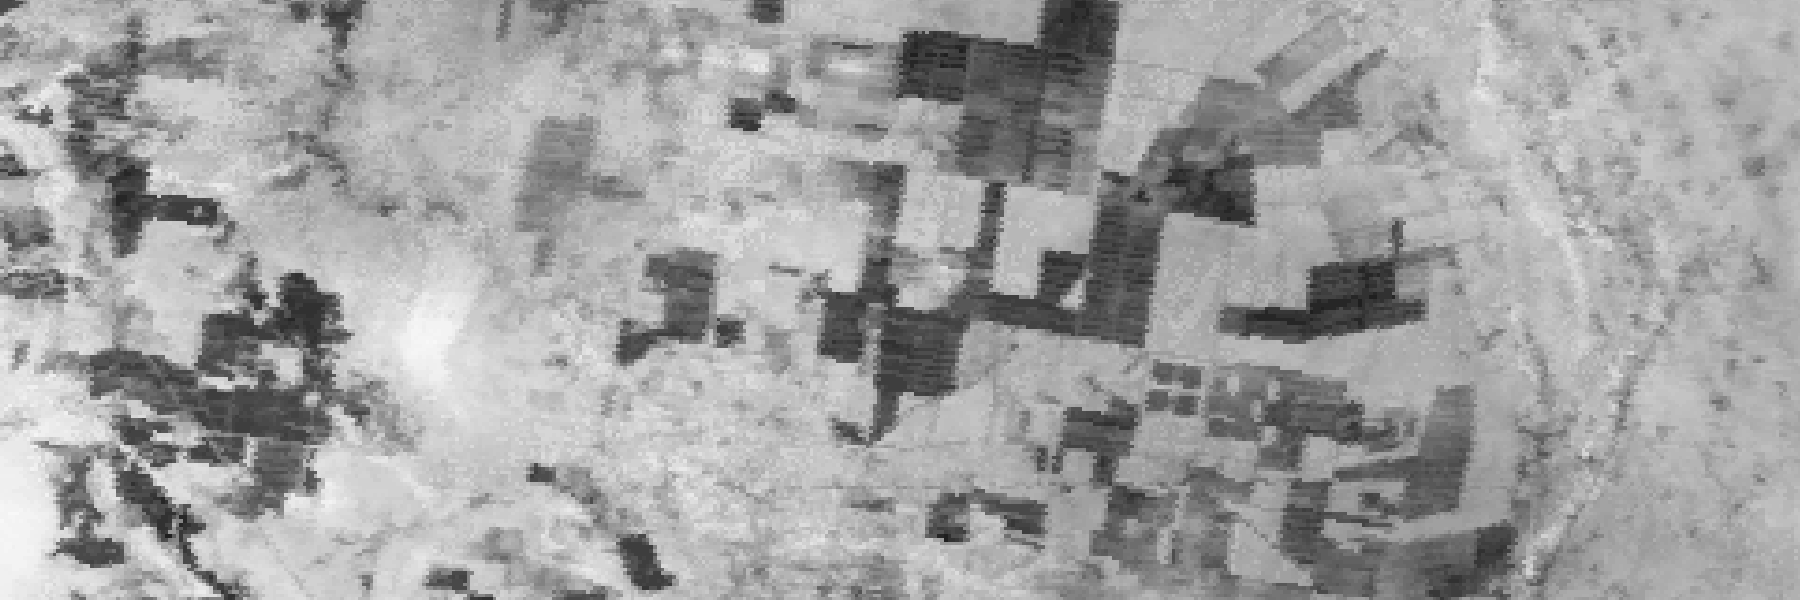
\includegraphics[width=\textwidth]{Graphics/vi_band1.png}
    \caption*{\formatdate{19}{12}{2013}}
    \label{subfig:vi_1}
  \end{subfigure}
  \\
  \vspace{0.125in}
  \begin{subfigure}[t]{\textwidth}
    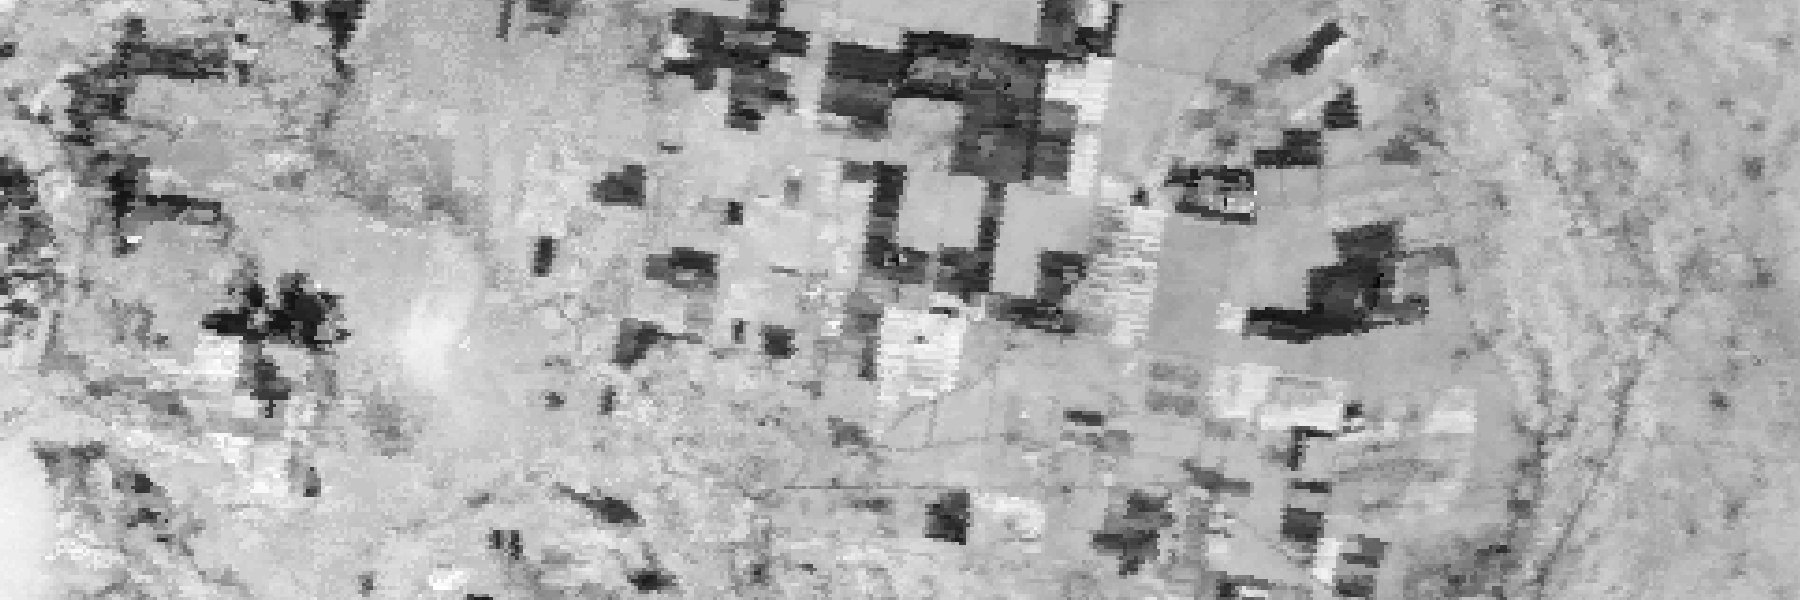
\includegraphics[width=\textwidth]{Graphics/vi_band4.png}
    \caption*{\formatdate{2}{2}{2014}}
    \label{subfig:vi_4}
  \end{subfigure}
  \\
  \vspace{.125in}
  \begin{subfigure}[b]{\textwidth}
    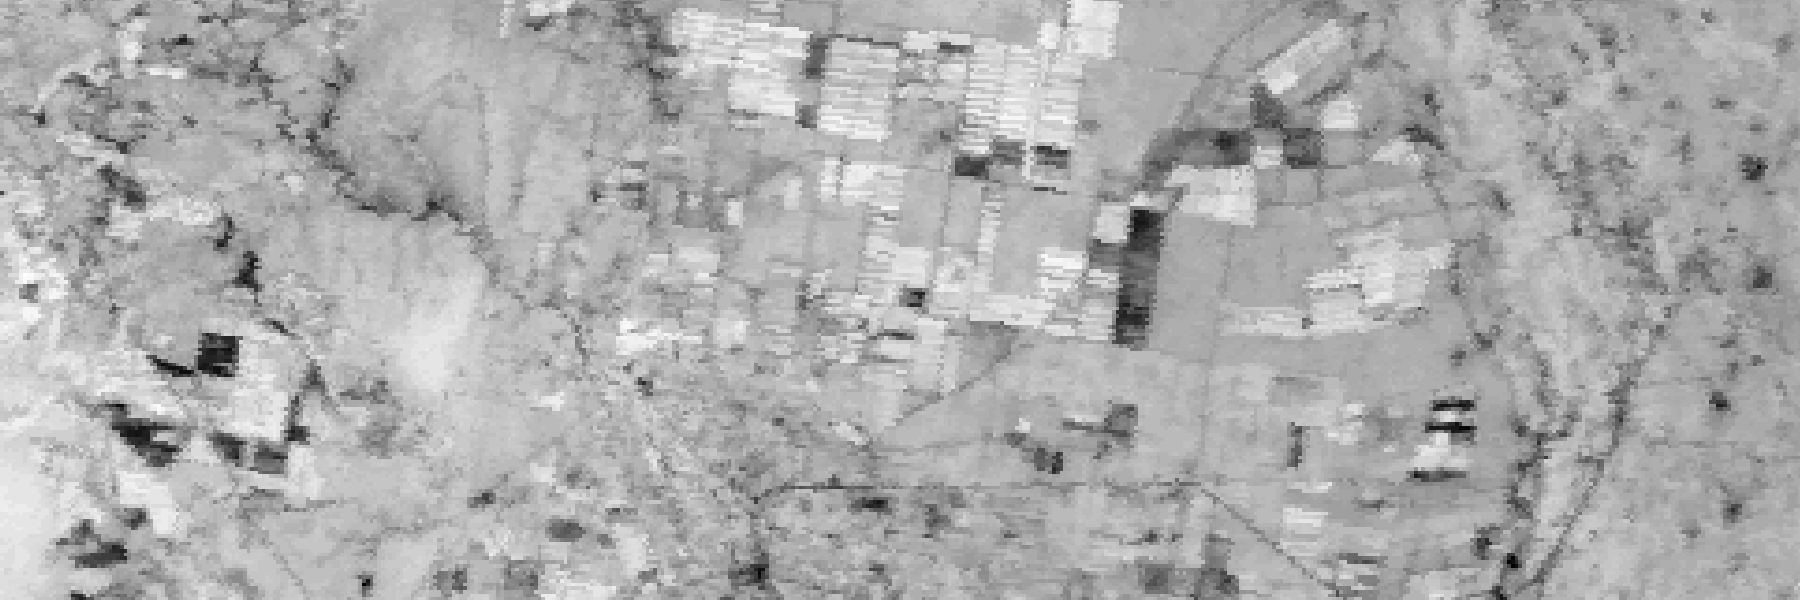
\includegraphics[width=\textwidth]{Graphics/vi_band8.png}
    \caption*{\formatdate{7}{4}{2014}}
    \label{subfig:vi_8}
  \end{subfigure}
  \caption{Example VI Progression}
  \label{fig:tsi}
  \medskip
  \small
  These MODIS NDVI images show the progression of VI values for a section of a MODIS tile containing the north half of Pellegrini and the surrounding area. The relative constant values for the forested areas stand in stark contrast to the fields, which predominately begin with low VI values in the first image, increasing as the crops mature to the greater values shown in the last image.
\end{ssfigure}
	
MODIS 16-day VI composite imagery from both the Terra and Aqua Earth Observing System (EOS) satellites is available from the Land Processes Distributed Active Archive Center (LPDAAC).\footnote{For those interested in working with MODIS data, the web address of LPDAAC is https://lpdaac.usgs.gov/, though data are not directly available from their servers without an exact link. I found the best tool for searching the available data was NASA’s Reverb|Echo web tool, at https://reverb.echo.nasa.gov/. Using this tool, one can get a list of links in a text file, and can use wget or curl to bulk download the files in the list.} Each MODIS satellite images the entire Earth daily: the Terra satellite makes its passes in the morning, while Aqua follows in the afternoon. This temporal resolution is the greatest advantage of the MODIS platform, as the likelihood of getting enough cloud-free data to develop a phenologic model is significantly increased over other common platforms like Landsat Thematic Mapper (TM) and Landsat Operational Land Imager (OLI), which only have repeat coverage every sixteen days. MODIS data, however, comes at the price of a reduced spatial resolution of 231 meters compared to Landsat’s 30-meter pixels.\footnote{Though the literature typically denotes MODIS data as 250-meter, the composite vegetation indices are actually 231-meter. However, to stay consistent with conventions, I will refer to the data as 250-meter.} At this resolution, crop mapping is restricted to medium farms and larger---those with fields of at least 250 meters square, though often a field must be up to two times larger in at least one dimension to ensure a pure pixel can be isolated. For the purposes of this investigation, however, this limitation is inconsequential, as small farms have a relatively minor impact on deforestation due to their size. Moreover, the crop of interest, GM soy, is only profitably grown using highly mechanized, input-intensive agricultural practices at very large scales \autocite{kaimowitz2001soybean}. Small fields do not have high enough yields to overcome the significant capital investment required.

LPDAAC creates the VI composites using the maximum VI value over the proceeding 16-day time period. The images are numbered by the day of the year (DOY) of the last date in the image's date range, so an image from DOY 17 is the composite of the images from \datenoyear{1}{1} through \datenoyear{17}{1}.\footnote{Following this pattern exactly will make the first image from the following year be from \datenoyear{4}{1}, but the MODIS composite numbering ``resets'' at the end of each year. Thus the image interval at the end of the year is shortened, allowing the next image to be produced \datenoyear{1}{1}, though it still covers the proceeding 16 days.} Both NDVI and EVI are included in the MODIS VI products, and require no preprocessing for immediate use (unless cloud cover is pervasive in the area). A chronological series of these VIs can be assembled into a time series image (TSI), which can then be used for processing.


\section{Crop Phenologies and Phenological Classification}
\label{methods:phenology-fitting}

\citeauthor{gu2010phenological} outlined that phenological statistics regarding vegetation development can be derived from a MODIS VI time-series, including ``start-of-season time, start-of-season NDVI, end-of-season time, end-of-season NDVI, maximum NDVI, maximum NDVI time, duration of season, amplitude of NDVI, and seasonal time integrated NDVI'' \mkbibparens{\citeyear[529]{gu2010phenological}}. A principal component analysis can then be used to extract the meaningful variation in the data.

Similarly, Wardlow, Egbert, et al. \autocites{wardlow2002discriminating}{wardlow2005state-level}{wardlow2007analysis}{wardlow2008large-area} showed that a decision tree classifier can be used to classify vegetation time-series data into increasingly refined categories until specific crop types are isolated and classified. By beginning with a basic land cover classification (e.g. forest, urban, agriculture), crops in the agriculture class can be broken down into winter and summer varieties using peaks in the vegetation index (winter wheat will peak earlier in the year than summer crops like corn and soy). Then, using training sites of known crop types defined by ground truth data, a final crop classification can be assigned by finding pixel values for key dates where like crops can be differentiated. That is, using the growing season in the Northern Hemisphere as an example, if from the training sites we know crop A has VI values between 0.7 and 0.8 on \datenoyear{26}{6} and between 0.5 and 0.6 on \datenoyear{29}{8}, while crop B is between 0.55 and 0.65 and 0.75 and 0.85 on the same dates, pixels in the summer crop class can be assigned one of these types by testing their pixel values on these dates. While the authors found this method to have about an 85 percent overall accuracy \autocite{wardlow2005state-level}, the downside of this method is that it requires training sites with previously-determined crop types to produce a classification, which can be time consuming and expensive to acquire.

\textcite{masialeti2010a-comparative} found that VI values from one year have a significant correlation with values from other years. Comparing the phenological curves of crops formed by the NDVI values from 2001 MODIS data \autocite[from][]{wardlow2005state-level} with those from 2005 MODIS data, the authors found the overall shape of each crop's curve is maintained year-to-year, with a subtle shift in the beginning of the curve (earlier or later planting), a scaling of the maximum of the curve (better or worse crop development), and and scaling of the spread of the curve (a longer or shorter growing season), depending on weather and other external variables (\autoref{fig:transformations}). They surmised, with a means to account for the shift and scaling of the curve, one could use VI values from one year to classify those from another.

\begin{ssfigure}
  \centering
  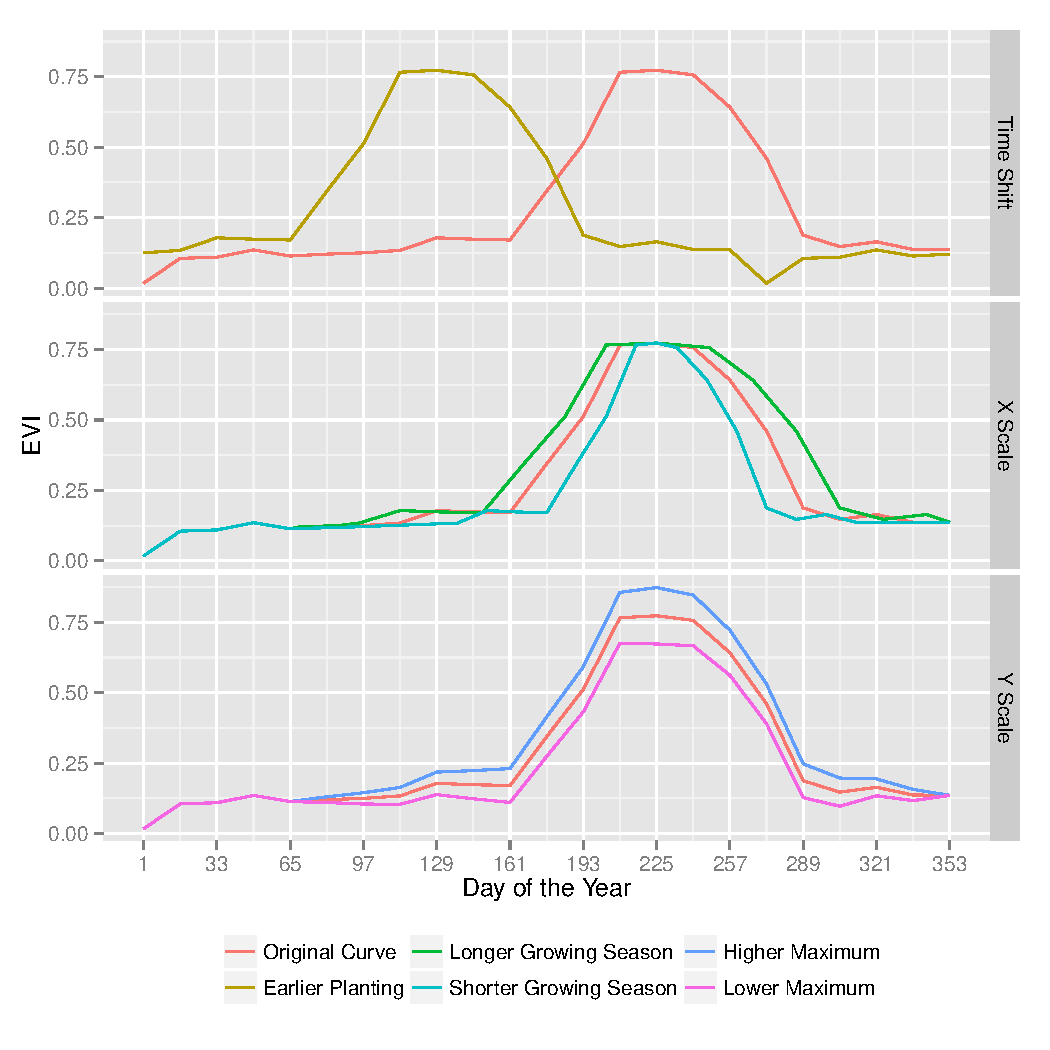
\includegraphics[width=\textwidth]{Graphics/transformations.pdf}
  \caption{Example Transformations of a Crop's VI Curve}
  \medskip
  \small
  The original signature was derived from soy in southwestern Kansas. The other signatures were arbitrarily adjusted to illustrate each of the possible transformations (the diagrams were created by me for illustration purposes).
  \label{fig:transformations}
\end{ssfigure}

Even without a mechanism to account for interannual differences, \textcite{brown2007multitemporal} used crop phenologies derived from multiple years of data to test four phenological classification methods. The authors fit the known phenologies to the unknown phenologies from other years by comparing the VI values throughout the growing season. The degree of likeness between a known VI curve and the unknown VI curve determined the classification. They showed that the best of the four classification methods was to find the sum of the square errors between the known and unknown curves (the SSE method, \citeauthor{brown2007multitemporal} pg. 131).

The similarities between the methods presented in \citeauthor{brown2007multitemporal} and hyperspectral remote sensing techniques are striking. Hyperspectral techniques compare known spectral \textit{signatures} from a signature library to the unknown pixel signatures in an image. One method, spectral feature fitting, uses a least-squares comparison reminiscent of SSE from \citeauthor{brown2007multitemporal} \autocites{solutions2013selected}{clark2003imaging}. The key difference between the two, besides comparing reflectance across time versus reflectance across the electromagnetic spectrum, is that spectral feature fitting does not require any training data from the processed image. All of the spectral signatures used for identification are from standardized spectral libraries, which contain the many spectra of different materials.

Accordingly, one goal of this study is to realize a method of vegetation classification using multi- or hyper-temporal imagery that does not require training data to be extracted from the imagery itself, rather relying on standard libraries of phenological curves---\textit{temporal} signatures---for different vegetation and non-vegetation land covers. A major challenge of this idea is that, unlike spectral signatures, temporal signatures are not necessarily consistent location to location, nor year to year as mentioned above. A viable classification method thusly must provide a way to transform the temporal signatures, within appropriate bounds, to match the horizontal scaling, vertical scaling, and time shifting of an unknown pixel before finding the degree of fit between the signature curve and the pixel curve.

\textcites{sakamoto2005a-crop}{sakamoto2010a-two-step} demonstrates a method using MODIS time-series data for use in finding key dates in a crop’s phenology, enabling better crop management strategies. Specifically, the authors’ two-step filter (TSF) method uses a wavelet transformation and a constrained minimization function to find a reference signature for a specific crop’s phenological development, and then fits that signature to known pixels of that crop type, finding the scaled dates of key transitions between developmental stages in the plants’ growth. This TSF method demonstrates that reference signatures can be fit to a pixel’s signature using a minimization function, accounting for the variations from the reference curve and the pixel curve.  This minimization method provides the means to account for the scaling and time shift differences, allowing previously-known temporal signatures (e.g. not from training sites) to be fit to pixel signatures in a TSI.

Specifically, from page 2151 of \textcite{sakamoto2010a-two-step}:
\begin{equation}
\label{eq:1}
  RMSE = \biggl[\frac{1}{365/s}\sum_{x\ =\ j(1),\ j(2)\ldots}^{n}\bigl(f\left(x\right)-g\left(x\right)\bigr)^{2}\biggr]^{\frac{1}{2}}
\end{equation}
where $n$ is the number of dates in the TSI, $f(x)$ is the temporal signature for a given pixel in a dataset, and $x$ is the DOY, as defined by $j(y)$:
\begin{subequations}
\label{eq:DOYcalc}
  \begin{align}
    j\left(~y\right) &= k\bigl(~i\cdot~s\left(~y - 1\right)\bigr) \label{eq:jofy}\\
    \text{where\ \ \ \ } k\left(~z\right) &=
    \begin{cases}
      z, & \mbox{if } z \leq 0\\
      \left(z\bmod~365\right)\bmod~i-1, & \mbox{if } z > 0
    \end{cases} \label{eq:kofz}
  \end{align}
\end{subequations}
such that $s$ is the interval of the imagery and $d$ is the starting date of the imagery. $g(x)$ in \autoref{eq:1} is given by:
\begin{equation}
\label{eq:gofx}
  g(x) = yscale\times~h\left(xscale\times(x + tshift)\right)
\end{equation}

Here, $x$ again is the DOY, $yscale$ and  $xscale$ are coefficients controlling the vertical and horizontal scaling of a reference signature $h(x)$, and $tshift$ is a constant representing the horizontal shift, in days, of $h(x)$. In other words, $yscale$ adjusts the reference signature to match the growth condition (i.e. maximum VI value) of the pixel (again, given by $f(x)$); $xscale$ adjusts the reference signature to match the pixel's growth cycle duration; and $tshift$, or time-shift, is the offset, in days, between the peak date of the reference signature and the peak date the pixel (see \autoref{fig:transformations}). Thus, if we minimize \autoref{eq:1} bounding $yscale$, $xscale$, and $tshift$  in $g(x)$ with reasonable values for each, we can calculate how well a given reference temporal signature $h(x)$ can be made to fit the pixel signature $f(x)$. Comparing a pixel's RMSE value from each of the reference signatures allows final classification; the signature with the lowest RMSE value has the best fit, and, of the tested signatures, provides the most probable identification.


\chapter{Study Areas}

This study will use agricultural areas in Kansas, USA for testing and verification of the phenological classification method and will apply the classification method to Pellegrini, Santiago del Estero, Argentina to test its effectiveness in subtropical South America.

\section{Kansas, USA}

The state of Kansas is one of the big agricultural producers of the US. As one of the plains states, it is relatively flat across much of its extent, making it well suited to large highly-mechanized agro-industrial operations. In 2012, the three most extensive crops in the state were wheat, corn, and soybeans (Table \ref{table:kansas}), which are also the most abundant crops in Pellegrini, Argentina. Additionally, Kansas has been the focus of a number of previous studies into the use of MODIS time-series for crop classification \autocites{wardlow2002discriminating}{wardlow2005state-level}{wardlow2007analysis}{wardlow2008large-area}, and has a very detailed and easily-accessible crop cover dataset in the form of the USDA CDL, making it a natural choice for a preliminary study area to test my method.

\begin{Spacing}{1.0}
\begin{table}
  \centering
  \caption[Most extensive crops in Kansas, 2012.]{Most extensive crops in Kansas, 2012\\~\autocite[adapted from][]{usda2013kansascrops}.}
  \label{table:kansas}
  \begin{tabular}{lcc}
    \toprule
     & Acreage (1,000 acres) & Production (1,000 units) \\
    \midrule
    Wheat & 9,100 & 382,200 \\
    Corn & 3,950 & 379,200 \\
    Soy & 3,810 & 83,820 \\
    All Hay & 2,750 & 4,340 \\
    All Forage & 2,750 & 4,545 \\
    Sorghum & 2,100 & 81,900 \\      
    \bottomrule
  \end{tabular}
\end{table}
\end{Spacing}


\section{Pellegrini, Santiago del Estero, Argentina}

Santiago del Estero, a province in Northwest Argentina, has an area of 136,351 square kilometers, about the same as Arkansas, but a population of about 874,000 \autocite{estadistica-y-c2010a}. The entire province is classified within the \textit{Parque Chaqueño} (Chaco forest), but the forested area has declined rapidly in the past fifteen years. Over the period 1998 to 2002, 306,055 hectares were deforested \autocite{secretaria-de-a2007informe}. From 2006 through 2011, a further 701,030 hectares of forest were lost, 283,669 of which were after the enacting of the OTBN \autocite{secreteria-de-a2012monitoreo}. Over both of these time periods Santiago del Estero experienced the highest levels of deforestation in all of Argentina.

The Department of Pellegrini is an administrative area in the Northwest corner of Santiago del Estero (Fig. \ref{fig:pellegrini}).\footnote{The Pellegrini boundary shapefile I obtained does not accurately reflect the bounds of the department on the ground. Particularly along the lengthy and straight northwestern edge, careful inspection of Figure \ref{fig:pellegrini} reveals a lack of registration between the vector geometry and the obvious boundary visible in the background image. When investigating some of my sample points along the northern and southern edges, I got strange looks and comments about how this or that field was not within Pellegrini, my supposed study area. So with this note, I want to acknowledge that I realize my study area is not actually the Department of Pellegrini proper, but an inaccurate representation as defined by the shapefiles from the Internet. I use this inaccurate representation to ensure consistency, to allow repeatability, and to simplify spatial analysis.} The department has an area of 6,944 square kilometers, a size slightly larger than the state of Delaware, and a 2010 population of only 20,514 \autocite{estadistica-y-c2010b}. The primary municipality of the department is Nueva Esperanza, with a population of about 4,500. The frontier nature of Pellegrini seems to have limited deforestation in the department for some time, but the push for land has increased the rate of deforestation. Over the years 2001 to 2005, only 5,968 hectares were found to be deforested (Volante 2005). From 2006 to 2011 the area deforested increased to 75,349 hectares, some 39,480 hectares cut after the enacting of the OTBN, a rate much higher than previously witnessed \autocite{secreteria-de-a2012monitoreo}. Of the area cleared post-OTBN, 2,181 hectares were in red areas, the highest clearing of that designation in the nation. The vast majority of clearing, however, was 29,796 hectares in yellow areas. While Pellegrini’s total deforestation during the period 2006 to 2011 was not the highest in Santiago del Estero, as both Moreno Department and Alberdi Department had higher total deforestation, as a percent of total land area Pellegrini’s deforestation occurred at a greater rate: 10.85 percent of Pellegrini’s land area was cleared versus 10.45 percent and 7.91 percent of Moreno and Alberdi, respectively.

\textcite{volante2005analisis} found Pellegrini's primary summer crop over the years 2000 to 2005 to be soy, averaging about 40,000 hectares cultivated per year. Corn was the second most frequent crop, occupying about 7,500 hectares per year. \textit{Poroto}, a generic term for many types of common beans, were the third most popular, averaging a total cultivation of about 2,500 hectares per year. The primary winter crop was wheat, though cultivation varied wildly from less than 10,000 hectares in 2002 to over 31,000 hectares in 2004.

\chapter{Data and Methods}

\section{Overview}

The purpose of this study is to develop a set of tools to allow the classification of agricultural crops 

\section{Composite Vegetation Indices and Time-Series Images}

The differentiation of crop types in remotely-sensed imagery is not a straightforward process. The use of a vegetation index (VI), such as the normalized difference vegetation index (NDVI) or the enhanced vegetation index (EVI), can help identify crops by their specific VI values in an image.

NDVI is a normalized ratio of the red and near-infrared bands, and can be expressed mathematically as:
\begin{equation}
  NDVI = \frac{\rho~_{NIR} - \rho~_{red}}{\rho~_{NIR} + \rho~_{red}}
\end{equation}
where $\rho~_{NIR}$ and $\rho~_{red}$ are the measured surface reflectance in their respective bands. As a ratio, the index minimizes multiplicative noise, but has issues with non-linearity and additive noise \autocite{huete2002overview}.

With advances in calibration, atmospheric correction, and other noise removal techniques which are integrated into the MODIS data processing workflow, a ratioing index is less necessary. The EVI was specifically developed for the MODIS platform to help correct some of the deficiencies of the NDVI. It has better sensitivity to high biomass, canopy structure, and leaf area, and less susceptibility to atmospheric degradation. EVI is calculated as:
\begin{equation}
  EVI = G\frac{\rho~_{NIR} - \rho~_{red}}{\rho~_{NIR} +  C_1\times\rho~_{red} - C_2 \times \rho~_{blue} + L}
\end{equation}
Again, each $\rho$ is the measured surface reflectance in the respective band, after complete or partial atmospheric correction. The blue band is used to "subtract" aerosol effects from the red band. Additionally, four coefficients are introduced: $G$ is the gain factor, $C_1$ and $C_2$ are used in the aerosol calculation, while $L$ "is the canopy background adjustment that addresses nonlinear, differential NIR and red radiant transfer through a canopy" \citereset\autocite[196]{huete2002overview}. The values of these coefficients as used in the MODIS EVI calculation are 2.5, 6.0, 7.5, and 1.0, respectively.

Some crops, such as soy and sugarcane, have very different spectral reflectance throughout their development and maturation, however others, such as soy and corn, can have very similar reflective curves, leading to overlapping VI ranges \autocite{price1994how-unique}. Such overlap can make it impossible to determine a crop type with specificity using traditional approaches; even using hyperspectral data, few differentiating characteristics between crops can hinder classification. To combat this, a time series of images can be used to find VI values throughout a year to develop a classification based on annual phenology rather than a single-date image \autocites{gu2010phenological}{wardlow2002discriminating}{wardlow2005state-level}{wardlow2007analysis}{wardlow2008large-area}{zhang2003monitoring}.
	
MODIS 16-day VI composite imagery from both the Terra and Aqua Earth Observing System (EOS) satellites is available from the Land Processes Distributed Active Archive Center (LPDAAC).\footnote{For those interested in working with MODIS data, the web address of LPDAAC is https://lpdaac.usgs.gov/, though data is not directly available from their servers without an exact link. I found the best tool for searching the available data was NASA’s Reverb|Echo web tool, at https://reverb.echo.nasa.gov/. Using this tool, one can get a list of links in a text file, and can use wget or curl to bulk download the files in the list.} Each MODIS satellite images the entire Earth daily: the Terra satellite makes its passes in the morning, while Aqua follows in the afternoon. This temporal resolution is the greatest advantage of the MODIS platform, as the likelihood of getting enough cloud-free data to develop a phenologic model is significantly increased over other common platforms like Landsat Thematic Mapper (TM) and Landsat Operational Land Imager (OLI), which only have repeat coverage every sixteen days. MODIS data, however, comes at the price of a reduced spatial resolution of 231 meters\footnote{Though the literature typically denotes MODIS data as 250-meter, the composite vegetation indices are actually 231-meter. However, to stay consistent with conventions, I will refer to the data as 250-meter.} compared to Landsat’s 30-meter pixels. At this resolution, crop mapping is restricted to medium farms and larger, though for the purposes of this investigation, this limitation is inconsequential, as small farms have a relatively minor impact on deforestation due to their size. Moreover, the crop of interest, soy, is 

LPDAAC creates the VI composites using the maximum VI value over the proceeding 16-day time period. The images are numbered by the day of the year (DOY) of the last date in the image, so an image from DOY 17 is the composite of the images from January 2 through January 17.\footnote{Following this pattern exactly will make the first image from the following year be from January 4, but the MODIS composite numbering "resets" at the end of each year. Thus the image interval at the end of the year is shortened, allowing the next image to be produced January 1, though it still covers the proceeding 16 days.} Both NDVI and EVI are included in the MODIS VI products, and require no preprocessing for immediate use (unless cloud cover is pervasive in the area).

For this study, I chose to classify the 2012 Kansas summer growing season and the 2014 Argentina summer growing season. I assembled the MODIS 16-day composite VI images into multi-date time-series images (TSI) covering the growth cycle of the summer crops, where each band in a TSI is a 16-day composite VI, and the bands are ordered consecutively. The Kansas summer TSI covered the date range DOY 97 through DOY 273, and was made with data from the Terra satellite. Prior to creating the TSIs, each of the 16-day composites was reprojected from the native MODIS sinusodial reference system using LPDAAC's MODIS Reprojection Tool [CITE THIS TOOL!!!!!]. I reprojected the Kansas data into the Albers Equal Area Conic projection for the contiguous USA using the 1983 North American Datum (NAD83) (WKID: 5070) to match the reference system of the USDA CDL.

In Argentina, as it is in the Southern Hemisphere and the seasons are inverted to those of the Northern hemisphere, the growing season shifts, as must the date range for the VI time-series. The TSI for Pellegrini must begin at the end of the proceeding year to adequately capture the entirety of the summer phenologies. To accomplish this, the time-series image for summer 2014 began with the 16-day composite image from DOY 345 of 2013 (or DOY −20 with reference to 2014) and ended with the image from DOY 105 of 2014. This specific date range was chosen based on information provided by local farmers to ensure coverage of the earliest planting and latest harvesting dates, as well as manual inspection of pixel signatures throughout the study area. Data through DOY 129 would have been preferred, but persistent clouds prevented using that late-date composite and necessitated the switch to the Aqua satellite's imagery. The Argentina composite images were reprojected with the UTM Zone 20S reference system (WKID: 32720).

\section{Crop Phenologies and Phenological Classification}

\citeauthor{gu2010phenological} outlined that phenological statistics regarding vegetation development can be derived from a MODIS VI time-series, including “start-of-season time (SOST), start-of-season NDVI (SOSN), end-of-season time (EOST), end-of-season NDVI (EOSN), maximum NDVI (MAXN), maximum NDVI time (MAXT), duration of season (DUR), amplitude of NDVI (AMP), and seasonal time integrated NDVI (TIN)” \mkbibparens{\citeyear[529]{gu2010phenological}}. A principal component analysis (PCA) can then be used to extract the meaningful variation in the data. Similarly, Wardlow, Egbert, et al. \autocites{wardlow2002discriminating}{wardlow2005state-level}{wardlow2007analysis}{wardlow2008large-area} showed that a decision tree classifier can be used to classify vegetation time-series data into increasingly refined categories until specific crop types are isolated and classified. By beginning with a basic land cover classification (e.g. forest, urban, agriculture), crops in the agriculture class can be broken down into winter and summer varieties using peaks in the vegetation index (winter wheat will peak earlier in the year than summer crops like corn and soy). Then, using training sites of known crop types defined by ground truth data, a final crop classification can be assigned by finding pixel values for key dates where like crops can be differentiated. That is, using the growing season in the Northern Hemisphere as an example, if from the training sites we know crop A has VI values between 0.7 and 0.8 on June 26 and between 0.5 and 0.6 on August 29, while crop B is between 0.55 and 0.65 and 0.75 and 0.85 on the same dates, pixels in the summer crop class can be assigned one of these types by testing their pixel values on these dates. While the authors found this method to have about an 85 percent overall accuracy \autocite{wardlow2005state-level}, the downside of this method is that it requires training sites with previously-determined crop types to produce a classification, which can be time consuming and expensive to acquire.

\textcite{masialeti2010a-comparative} found that VI values from one year have a significant correlation with values from other years. Comparing the phenological curves of crops formed by the NDVI values from 2001 MODIS data \autocite[from][]{wardlow2005state-level} with those from 2005 MODIS data, the authors found the overall shape of each crop's curve is maintained year-to-year, with a subtle shift in the beginning of the curve (earlier or later planting), a scaling of the maximum of the curve, and and scaling of the spread of the curve (a longer or shorter growing season), depending on weather and other external variables (Fig. \ref{fig:transformations}). They surmised, with a means to account for the shift and scaling of the curve, one could use VI values from one year to classify those from another.

\begin{figure}
  \centering
  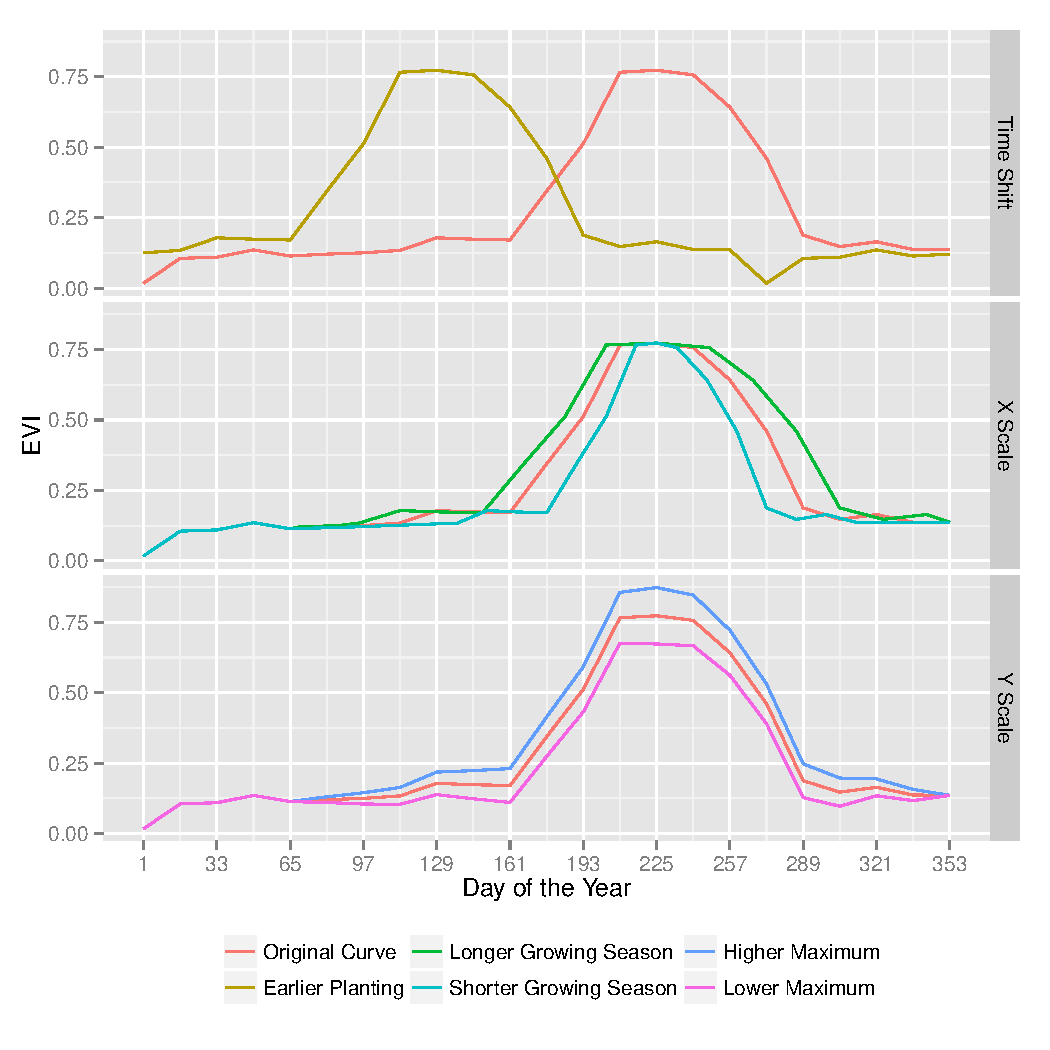
\includegraphics[width=\textwidth]{Graphics/transformations.pdf}
  \caption{Examples of transformations of a crop's VI curve due to interannual variations in growing conditions. The original curve was derived from soy in southwestern Kansas. The other curves were arbitrarily adjusted to illustrate each of the possible transformations.}
  \label{fig:transformations}
\end{figure}

Even without a mechanism to account for interannual differences, \textcite{brown2007multitemporal} used crop phenologies derived from multiple years of data to test four phenological classification methods. The authors fit the known phenologies to the unknown phenologies from other years by comparing the VI values throughout the growing season. The degree of likeness between a known VI curve and the unknown VI curve determined the classification. They showed that the best of the four classification methods was to find the sum of the square errors between the known and unknown curves (the SSE method, pg. 131).

The similarities between the methods presented in \citeauthor{brown2007multitemporal} and hyperspectral remote sensing techniques are striking. Hyperspectral techniques compare known spectral \textit{signatures} from a signature library to the unknown pixel signatures in an image. One method, spectral feature fitting, uses a least-squares comparison reminiscent of \citeauthor{brown2007multitemporal}s’ SSE \autocite{solutions2013selected}{clark2003imaging}. The key difference between the two, besides comparing reflectance across time versus reflectance across the electromagnetic spectrum, is that spectral feature fitting does not require any training data from the processed image. All of the spectral signatures used for identification are from standardized spectral libraries, containing many spectra of different materials.

Accordingly, one goal of this study is to realize a method of vegetation classification using multi- or hyper-temporal imagery that does not require training data to be extracted from the imagery itself, rather relying on standard libraries of \textit{temporal signatures} for different vegetation and non-vegetation land covers. A major challenge of this idea is that, unlike spectral signatures, temporal signatures are not necessarily consistent location to location, nor year to year as mentioned above. A viable classification method thusly must provide a way to transform the temporal signatures, within appropriate bounds, to match the horizontal scaling, vertical scaling, and time shifting of an unknown pixel before finding the degree of fit between the signature curve and the pixel curve.

\textcites{sakamoto2005a-crop}{sakamoto2010a-two-step} demonstrates a method using MODIS time-series data for use in finding key dates in a crop’s phenology, enabling better crop management strategies. Specifically, the authors’ two-step filter (TSF) method uses a wavelet transformation and a constrained minimization function to find a reference signature for a specific crop’s phenological development, and then fits that signature to known pixels of that crop type, finding the scaled dates of key transitions between developmental stages in the plants’ growth. This TSF method demonstrates that reference signatures can be fit to a pixel’s signature using a minimization function, accounting for the variations from the reference curve and the pixel curve.  This minimization method provides the means to account for the scaling and time gift differences, allowing previously-known temporal signatures (i.e. not from training sites) to be fit to pixel signatures in a VI TSI.

Specifically, from page 2151 of \textcite{sakamoto2010a-two-step}:

\begin{equation}
\label{eq:1}
  RMSE = \biggl[\frac{1}{365/s}\sum_{x=j(0), j(1)…}^{n}\bigl(f\left(x\right)-g\left(x\right)\bigr)^{2}\biggr]^{\frac{1}{2}}
\end{equation}

where $n$ is the number of dates in the TSI, $f(x)$ is the phenological curve for a given pixel in a dataset, and $x$ is the DOY, as defined by $j(y)$:

\begin{subequations}
\label{eq:DOYcalc}
  \begin{align}
    j\left(~y\right) &= k\bigl(~i\cdot~s\left(~y - 1\right)\bigr) \label{eq:jofy}\\
    \text{where\ \ \ \ } k\left(~z\right) &=
    \begin{cases}
      z, & \mbox{if } z \leq 0\\
      \left(z\bmod~365\right)\bmod~i-1, & \mbox{if } z > 0
    \end{cases} \label{eq:kofz}
  \end{align}
\end{subequations}

such that $s$ is the interval of the imagery and $d$ is the starting date of the imagery. $g(x)$ in Equation \ref{eq:1} is given by:
\begin{equation}
\label{eq:gofx}
  g(x) = yscale\times~h\left(xscale\times(x_0 + tshift)\right)
\end{equation}

Here, $yscale$ and  $xscale$ are coefficients controlling the vertical and horizontal scaling of a reference signature $h(x_0)$, and $tshift$ is a constant representing the horizontal shift, in days, of $h(x_0)$ (Fig. \ref{fig:transformations}). $x_0$ is the day of year in the shape model. Thus, if we minimize eq. 3 bounding $yscale$, $xscale$, and $tshift$  in $g(x)$ with reasonable values for each, we can calculate how well a given reference temporal signature $h(x_0)$ can be made to fit the pixel signature $f(x)$ from Equation \ref{eq:1}. Comparing a pixel's RMSE fit value from each of the reference signatures allows final classification; the signature with lowest RMSE value has the best fit, and, of the tested signatures, provides the most probable identification.
\subsection*{Research Timeline}

I hope to have finished the classification algorithm by the beginning of winter term 2014.  At that point, I will run the testing on the Kansas sample areas to find the best reference curves. Once that testing is completed, I will use those curves to classify MODIS data of Pellegrini from the 2012 -- 2013 growing season. This will provide me with a rough picture of the crop cover my method will find for 2013 -- 2014, and from this I can use a stratified random sampling technique to better ensure my ground truthing will contain sufficient sample points in each land cover class. In March 2014 I plan to do fieldwork in Pellegrini to collect the ground truth data for these points. I have chosen the month of March specifically because it is in the middle of the summer growing season, and I can get ground truth data for summer crop identification as the crops are growing. Winter crops, such as winter wheat, will need to be verified by inquiring with field owners, or confirmed by visual interpretation of Landsat imagery. In spring term 2014, I will classify 2013 -- 2014 data for Pellegrini, calculate the accuracy using the ground truth acquired in March, and begin writing. I plan to finish my work and writing over summer 2014 and present fall 2014.

\chapter{Results}
\section*{Preliminary Results}
\label{sec:prelim}

To this point, I have been able to create scripts to import and assemble my multi-date images; to sample images and generate mean reference curves of the VI values for soy, corn, and wheat (Fig. \ref{fig:curves}; and to take said reference curves and generate an image for each crop, of which the pixel values are the RMSE after constrained minimization, and an image with the best fit for each pixel (Fig. \ref{fig:testing1}). For script development I am using MODIS 16-day EVI data from 2012. I have not completed the computation of the confidence scores of any given classification (a la fuzzy classification), but, for the sake of exploring this initial output, I used a threshold of .08 RMSE and classified the image according to the best fit. That is, for any pixels which had an RMSE of .08 or less for one or more of the crops tested, I used the best fit image values for those pixels as the values for classification (Fig. \ref{subfig:classification1}). I used the USDA CDL for 2012, resampled to 250 meter pixels with the majority value (Fig. \ref{subfig:CDL}), to check my classification. Building a confusion matrix for all of the pixels in the image resulted in Table \ref{table:acc}. As shown, the accuracies for each of the crops ranged between 60 percent and 70 percent, with an overall accuracy of 63 percent, though the kappa value is somewhat low at 0.44. Nonetheless, considering this is the unoptimized algorithm with an arbitrary threshold value, I believe my results suggest this classification method to have potential.

\begin{figure}
  \centering
  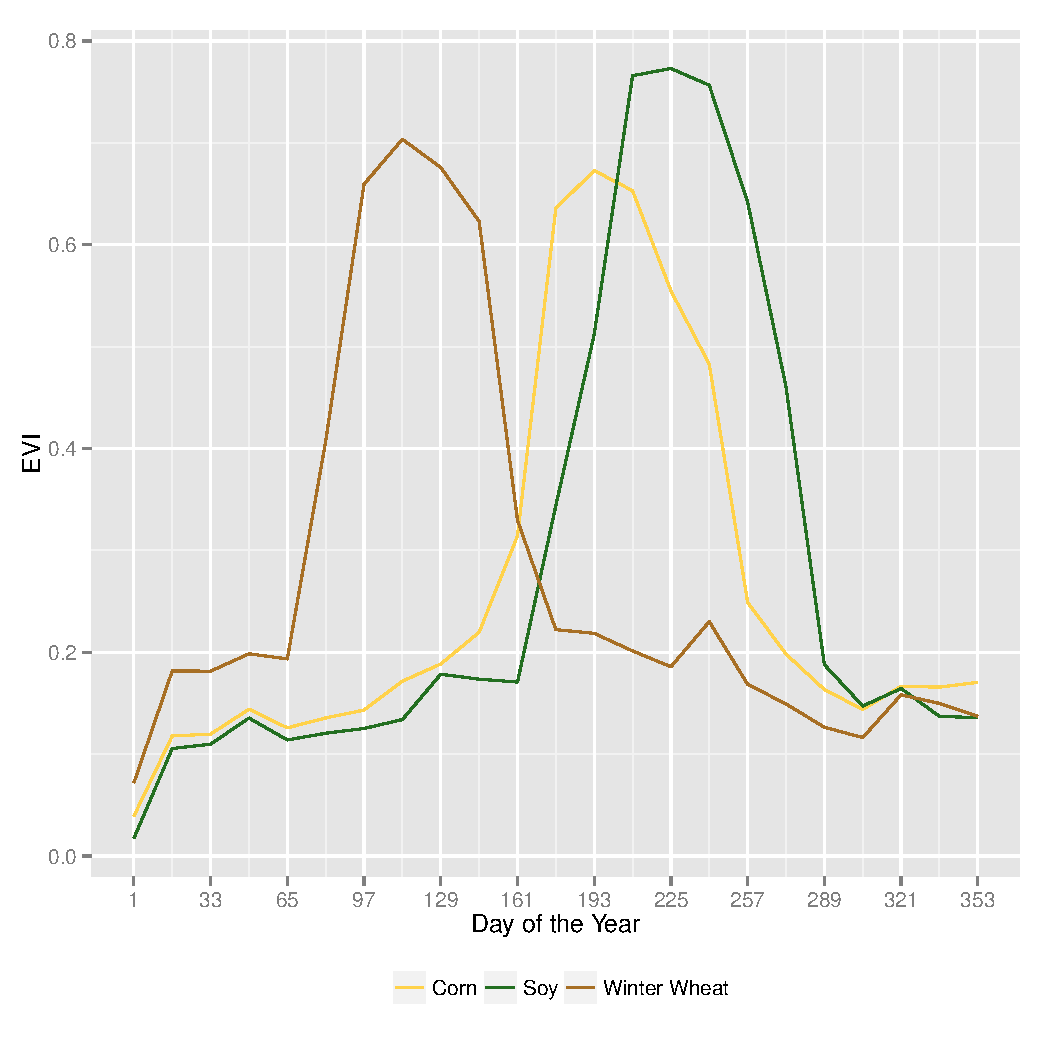
\includegraphics[width=\textwidth]{Graphics/cropCurves.pdf}
  \caption{Mean phenological curves found for corn, soy, and winter wheat. Each curve is generated from the mean EVI values of four pixels of the respective crop from an initial test area in 2012 Kansas data.}
  \label{fig:curves}
\end{figure}

\begin{figure}
  \centering
  \begin{subfigure}[b]{.45\textwidth}
    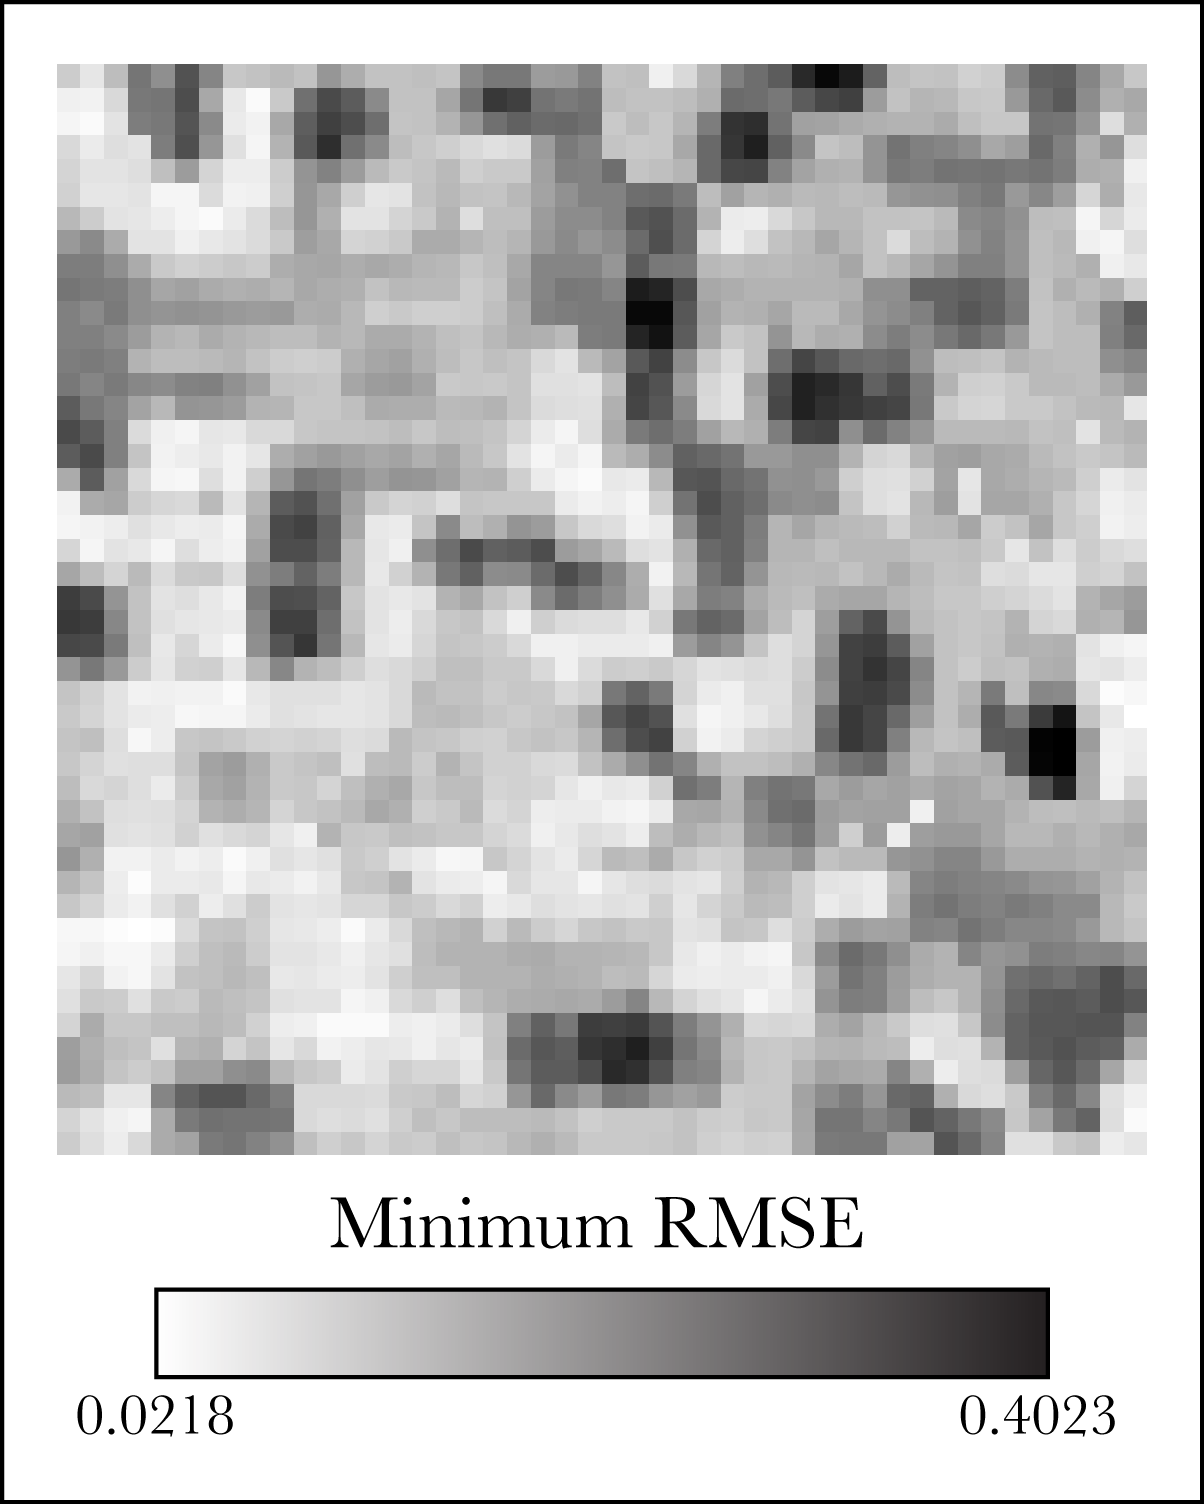
\includegraphics[width=\textwidth]{Graphics/corn1_edited.png}
    \caption{Fit of corn reference curve.}
    \label{subfig:corn1}
  \end{subfigure}
  \quad
  \begin{subfigure}[b]{.45\textwidth}
    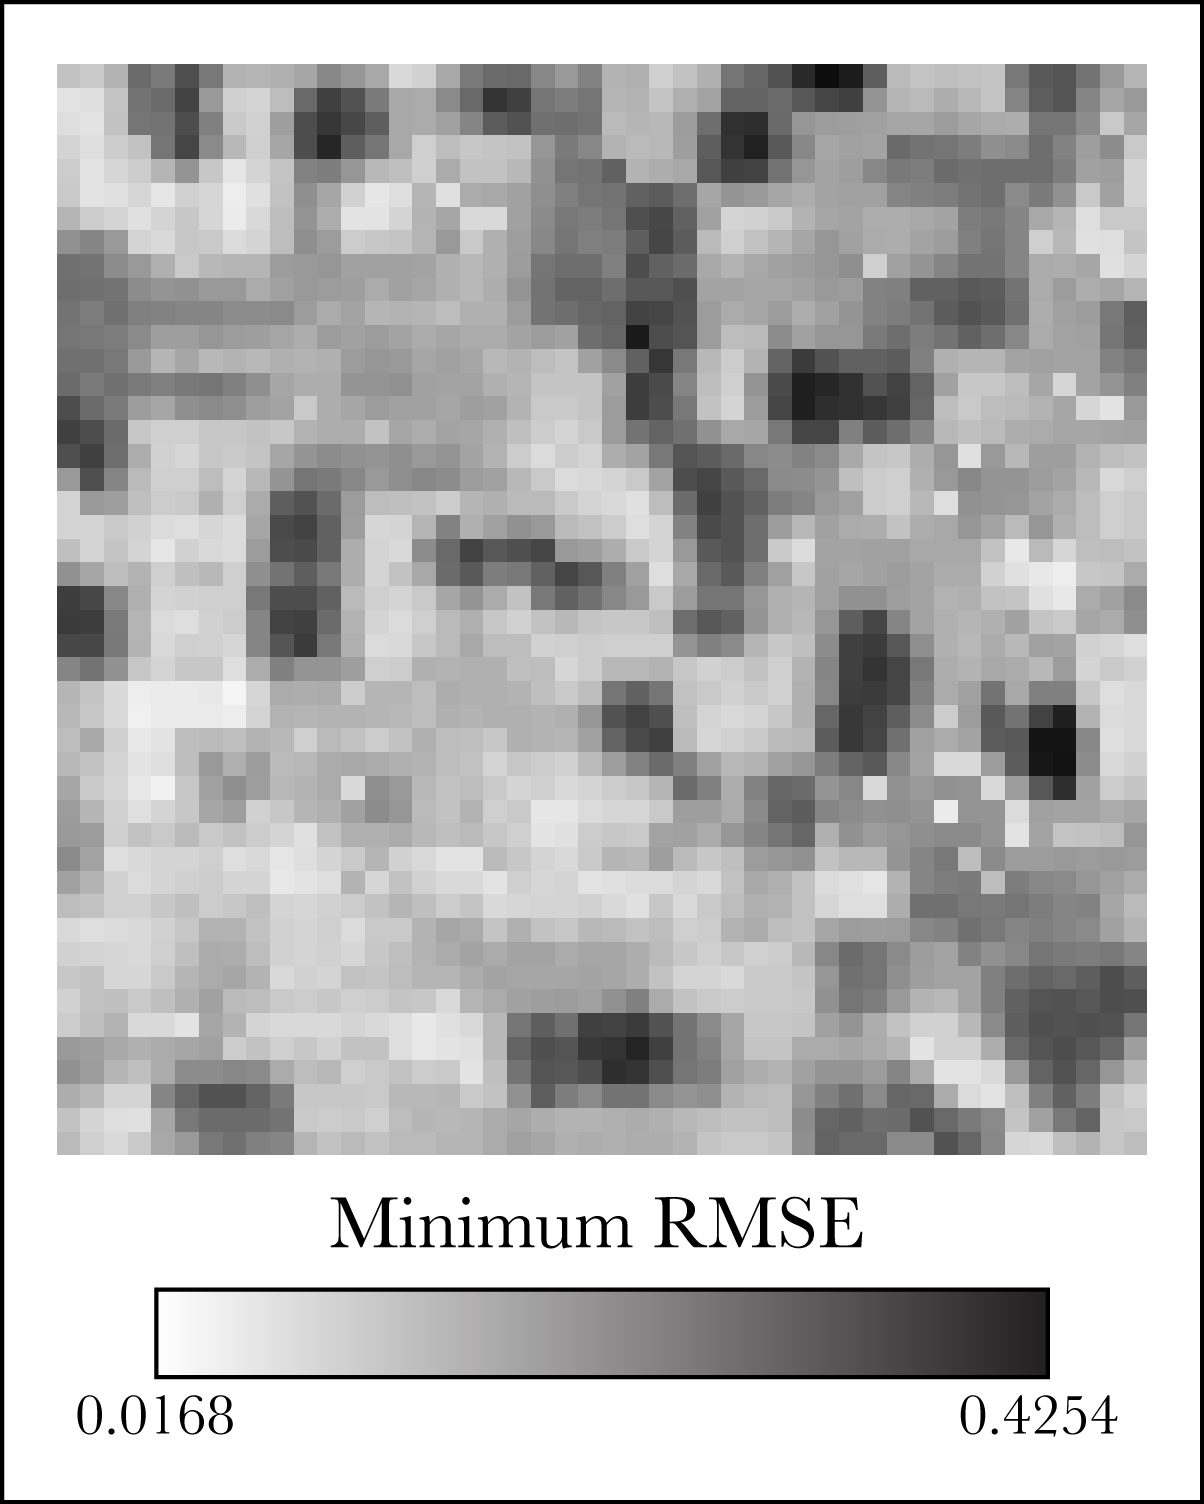
\includegraphics[width=\textwidth]{Graphics/soy1_edited.png}
    \caption{Fit of soy reference curve.}
    \label{subfig:soy1}
  \end{subfigure}
  \\
  \vspace{.25in}
  \begin{subfigure}[b]{.45\textwidth}
    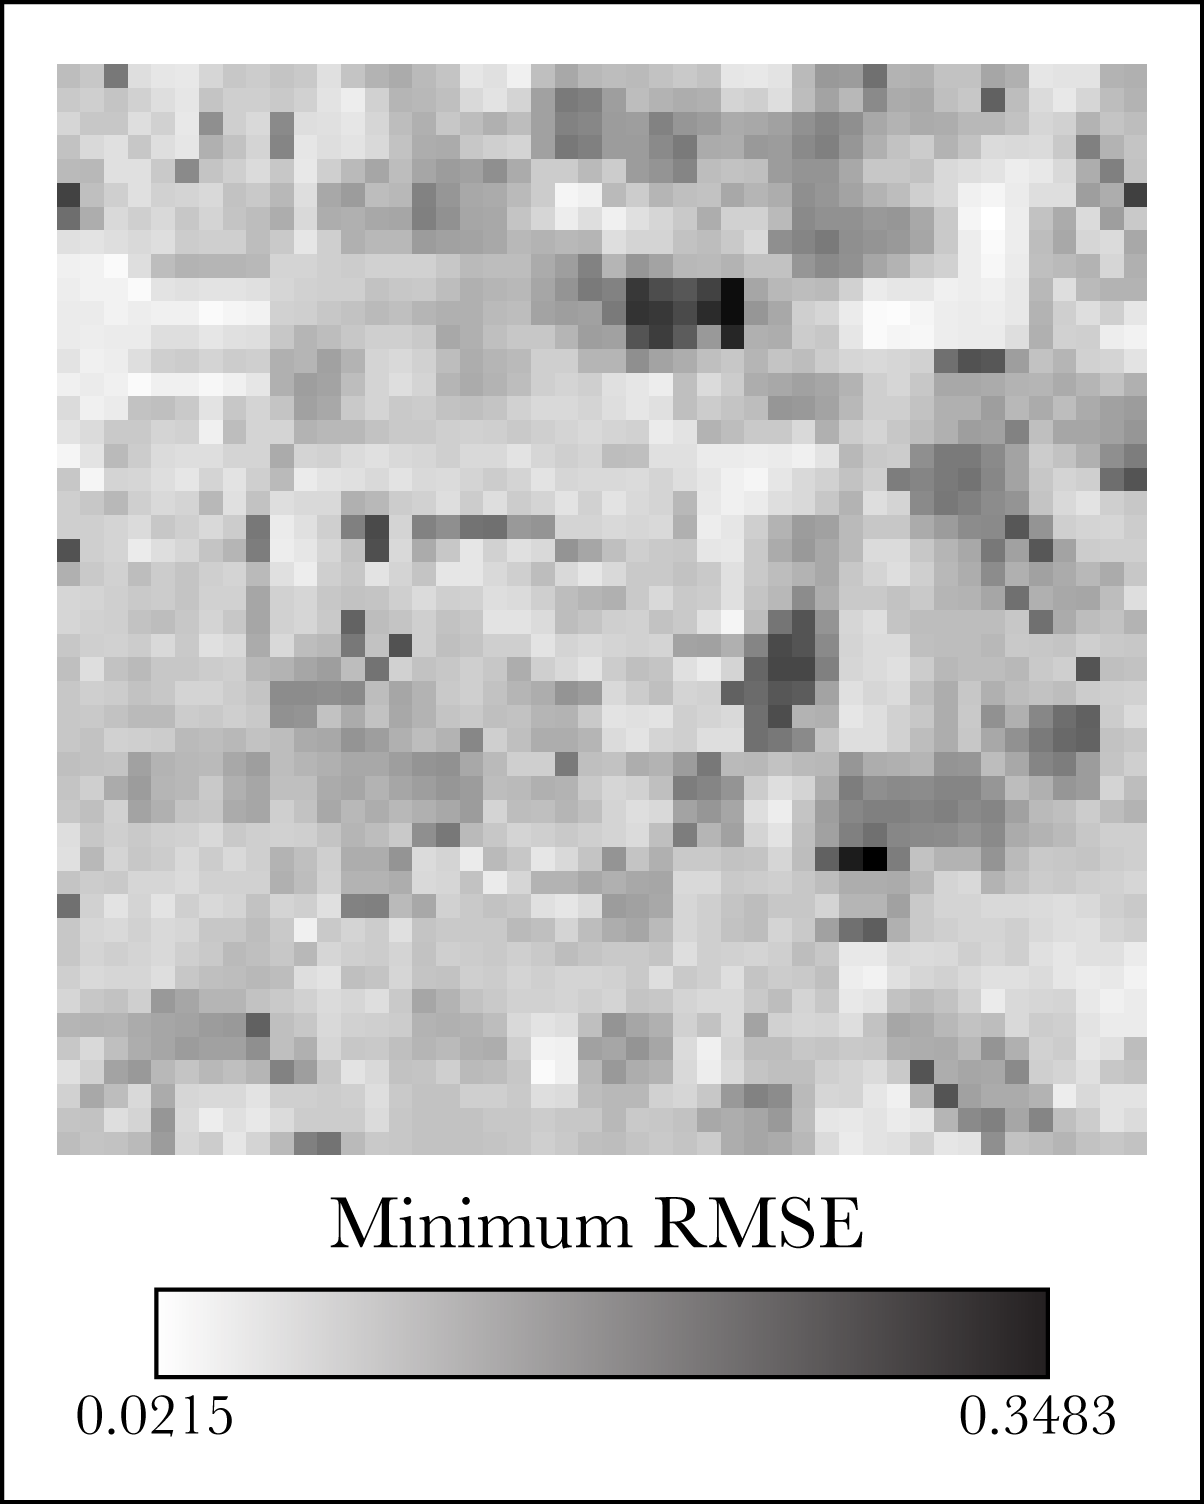
\includegraphics[width=\textwidth]{Graphics/wheat1_edited.png}
    \caption{Fit of wheat reference curve.}
    \label{subfig:wheat1}
  \end{subfigure}
  \quad
  \begin{subfigure}[b]{.45\textwidth}
    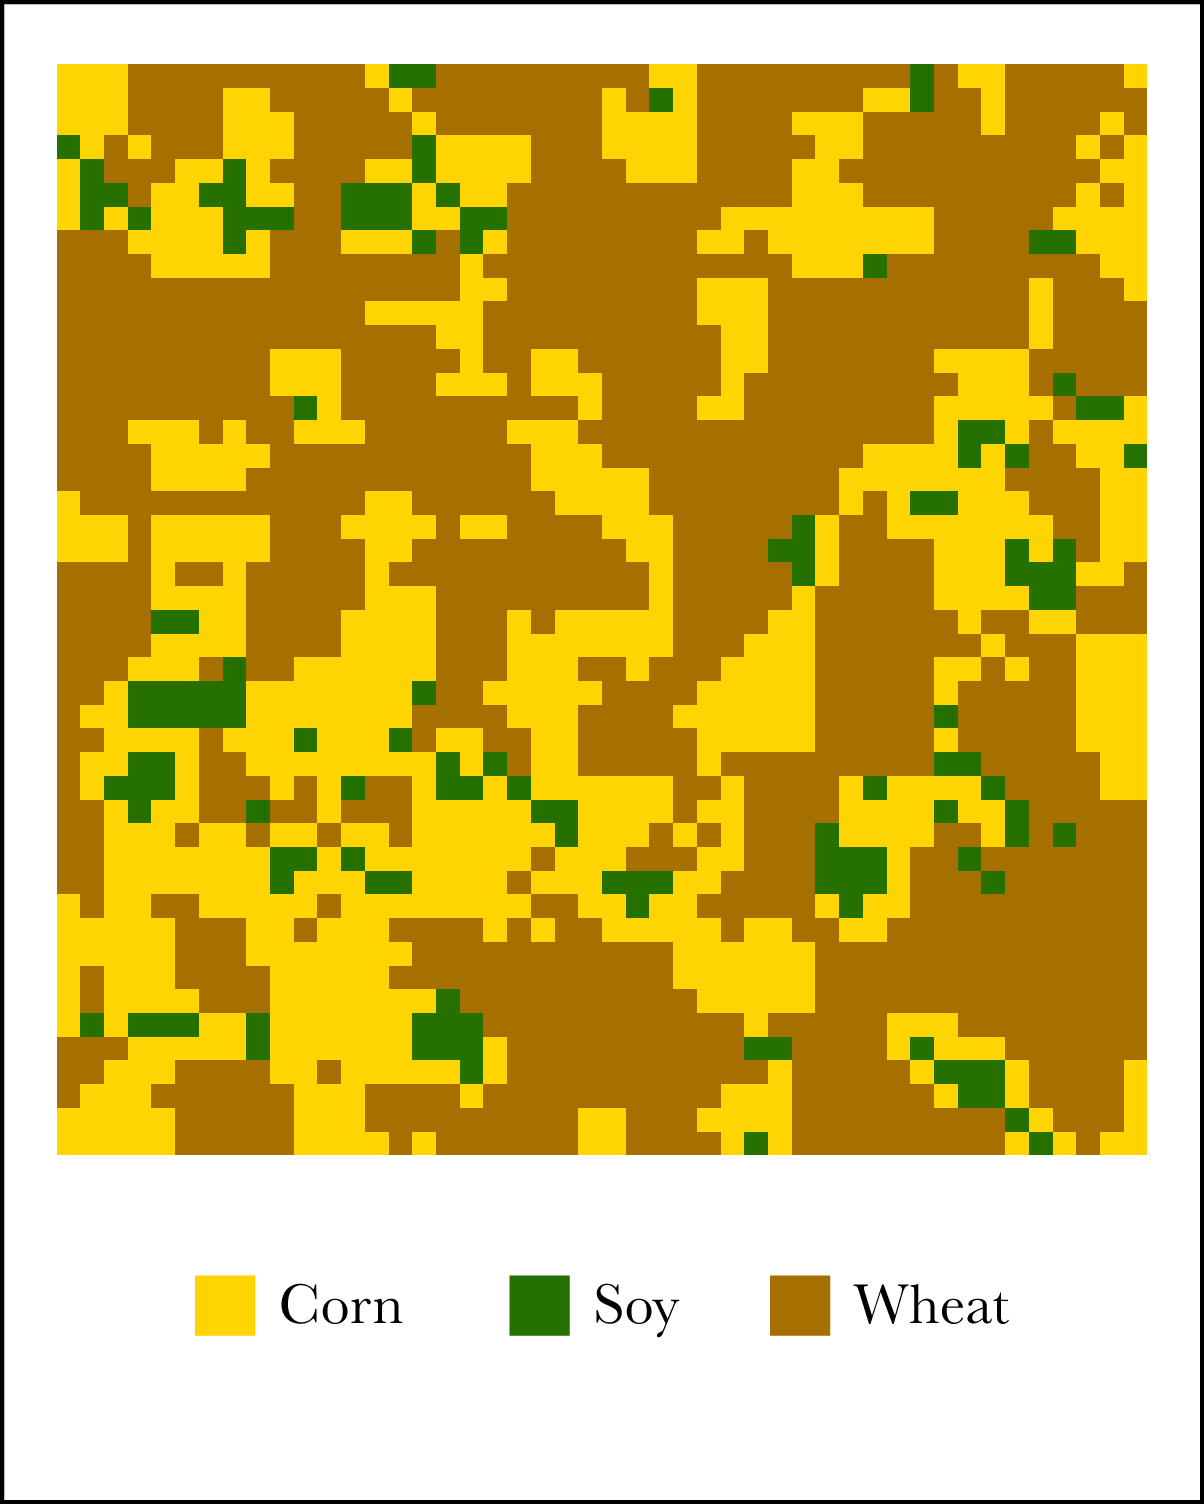
\includegraphics[width=\textwidth]{Graphics/bestfit_edited.png}
    \caption{Best fit image.}
    \label{subfig:bestfit1}
  \end{subfigure}
  \caption{Initial test results.}
  \label{fig:testing1}
\end{figure}


\begin{figure}
  \centering
  \begin{subfigure}[b]{.45\textwidth}
    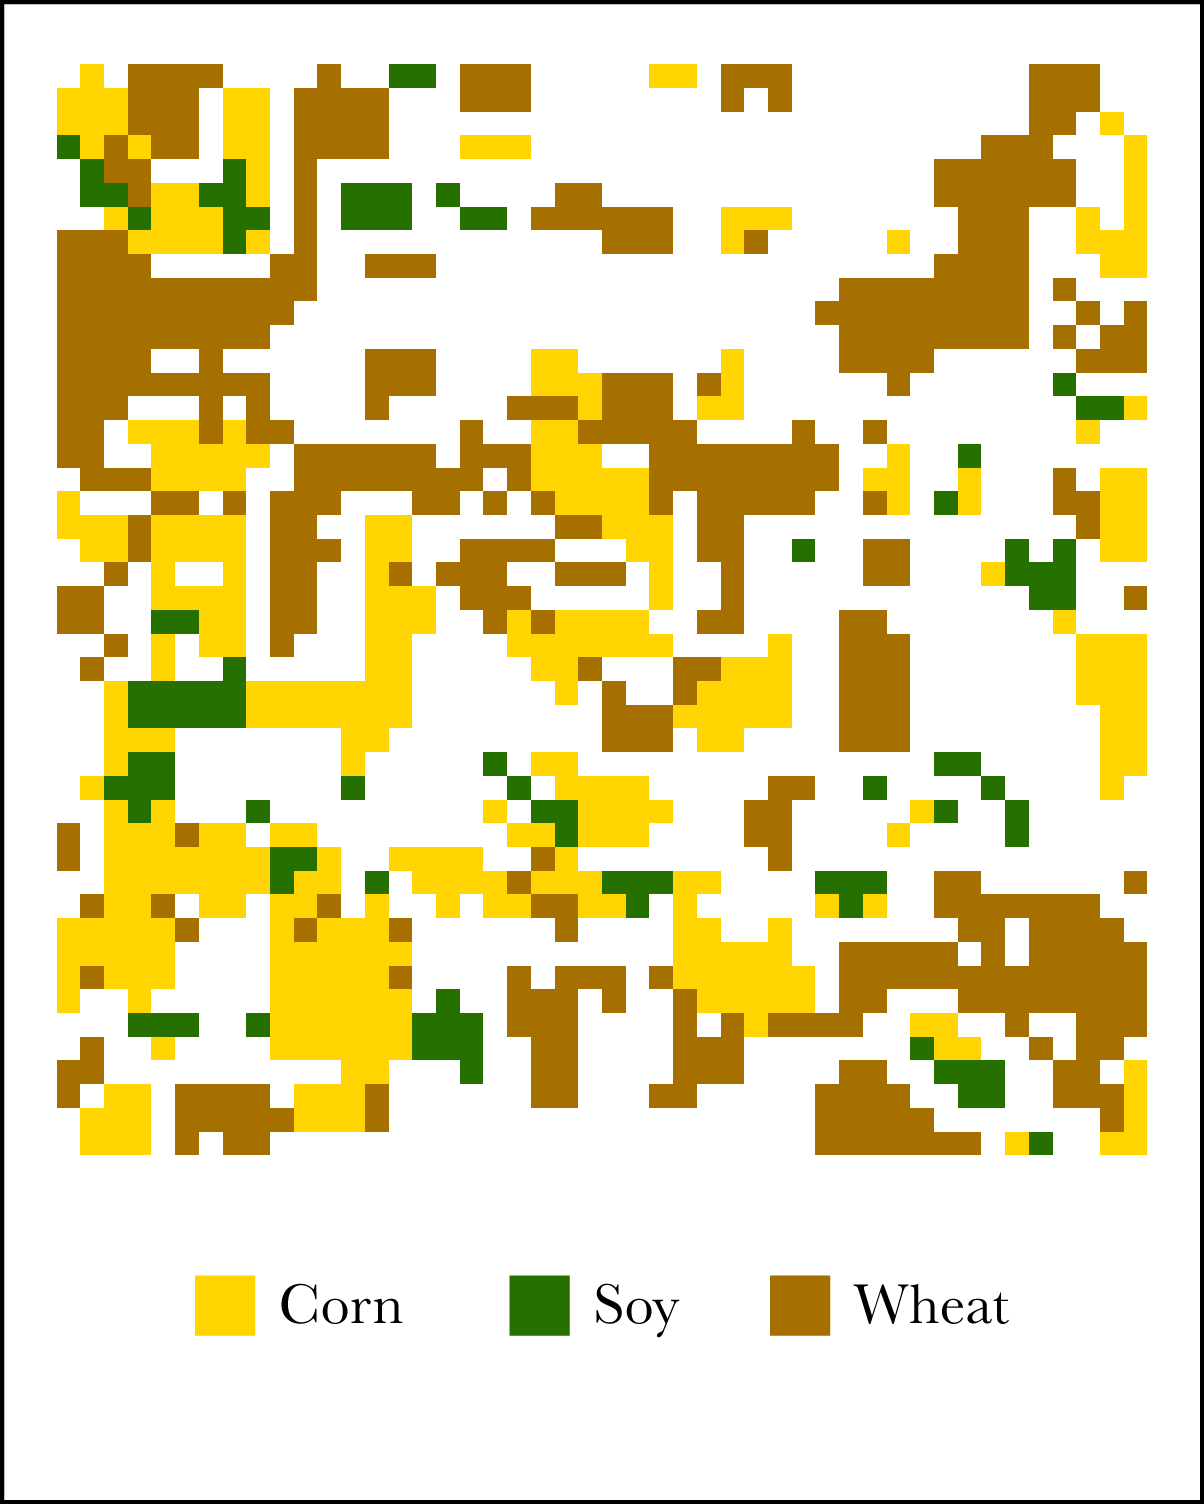
\includegraphics[width=\textwidth]{Graphics/classification1_edited.png}
    \caption{Initial classification of corn, soy, and wheat.}
    \begin{minipage}{.1cm} %fills vertical space to vertical align both subfigures
      \vfill
    \end{minipage}
    \label{subfig:classification1}
  \end{subfigure}
  \quad
  \begin{subfigure}[b]{.45\textwidth}
    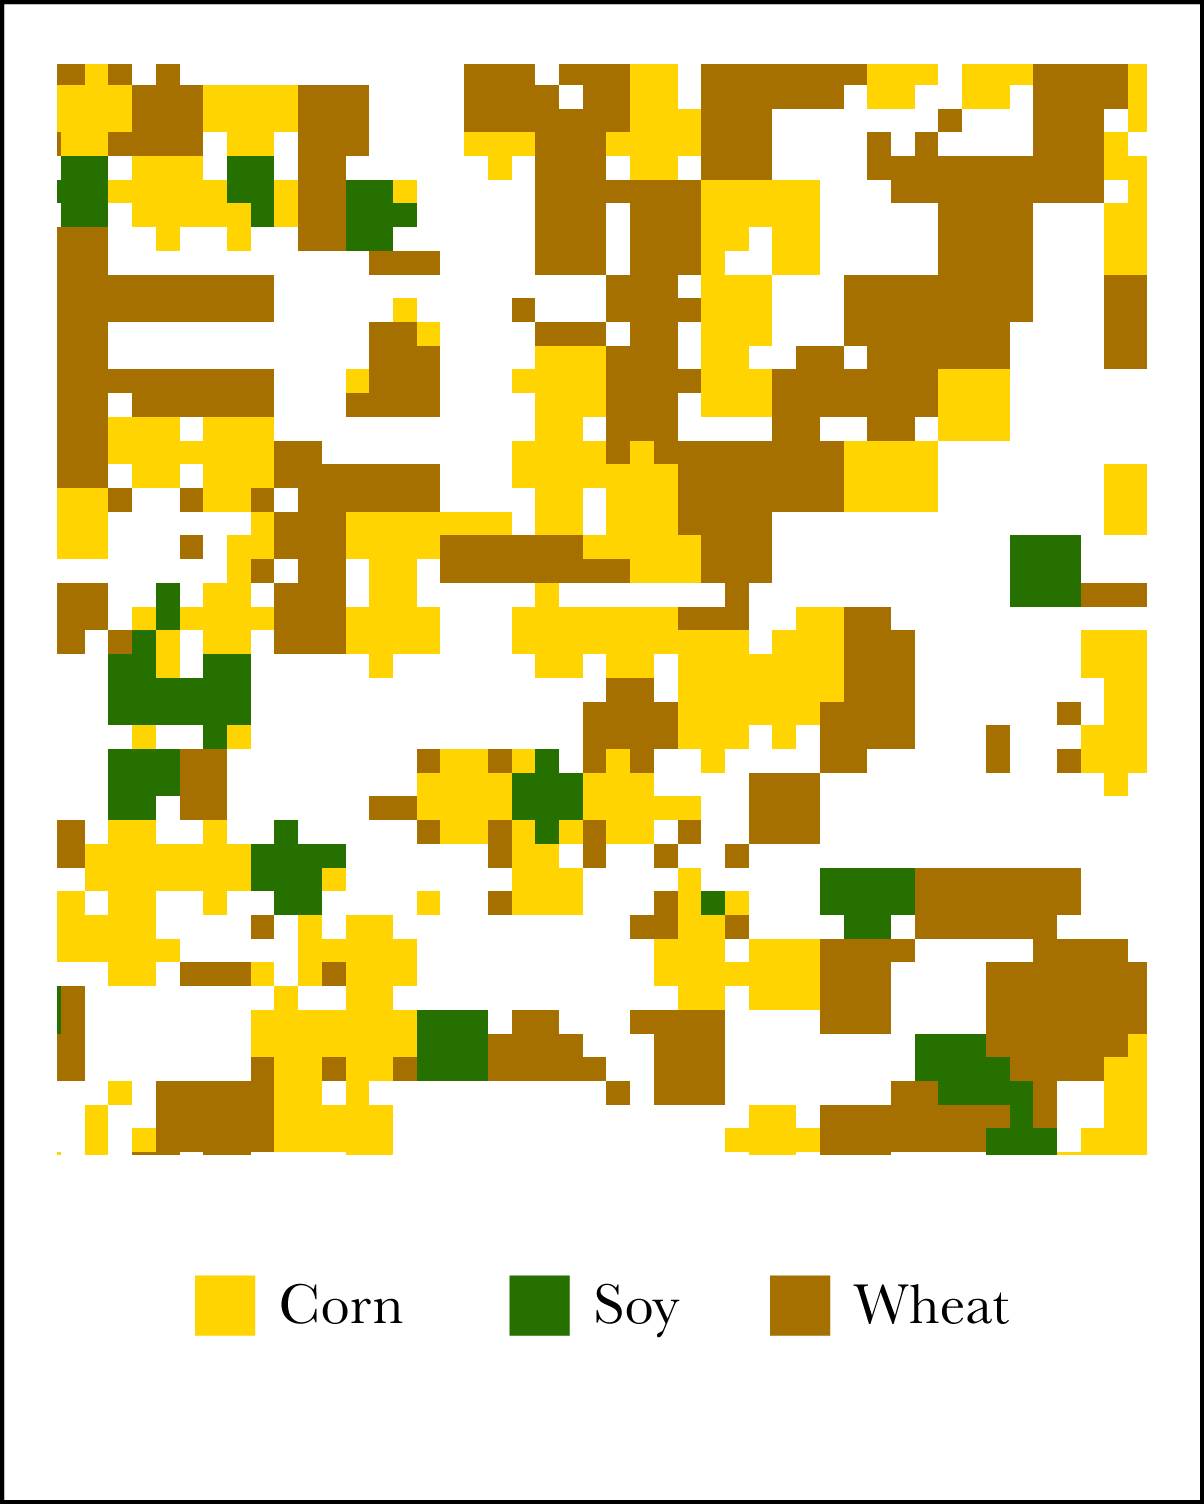
\includegraphics[width=\textwidth]{Graphics/cdl_rsmp_edited.png}
    \caption{2012 USDA CDL, resampled to 250m pixels to match MODIS data.}
    \label{subfig:CDL}
  \end{subfigure}
  \caption{Initial classification and ground truth}
  \label{fig:classification}
\end{figure}


\begin{table}
  \centering
  \caption{Accuracy assessment of the initial results.}
  \label{table:acc}
  \begin{tabular}{rcccccc}
    \toprule
     & Corn & Soy & Wheat & Other & Total & User Accuracy \\
    \midrule
    Corn & 260 & 22 & 6 & 103 & 391 & 67\% \\
    Soy & 10 & 59 & 1 & 29 & 99 & 60\% \\
    Wheat & 33 & 0 & 354 & 127 & 514 & 69\% \\
    Other & 174 & 27 & 241 & 670 & 1112 & 60\% \\
    Total & 477 & 108 & 602 & 929 & 2116 \\
    Producer Accuracy & 55\% & 55\% & 59\% & 72\% \\
     &  &  &  &  &  & Overall: 63\%\\
     &  &  &  &  &  & Kappa: 0.443 \\      
    \bottomrule
  \end{tabular}
\end{table}


\section*{Anticipated Outcomes}

Upon the completion of my research, I expect to have a working tool which can be used as an economical and effective means of crop classification. With the results of my testing, I will know how changes in the generation of the reference curves effects the results of the classifier. Using this tool and knowledge, I will generate crop maps of my study areas, and quantify their accuracies. The results of this study should be of value to those working in the field of remote sensing and those investigating LULC change, particularly in regard to deforestation and agriculture. I hope this work will be the basis for future investigations into soy's role in Argentina's deforestation.



















\clearpage
%\newpage
\section*{Appendix 1 -- Project Code}

The code for this project is all written in python version 2.7.5, and has various dependencies, listed below:

\begin{spacing}{1}
\begin{itemize}
  \item[--] GDAL 1.8 with python bindings
  \item[--] Scipy 0.12.0
  \item[--] Numpy 1.6.2
\end{itemize}
\end{spacing}

The project is currently split into three scripts: one to import the VI images and build the composite multi-date VI image (Script 1); one to extract the mean reference curves from pixels of known crop type in an image (Script 2, page \pageref{script2}); and one to use minimization to fit said reference curves to pixel curves, writing the RMSE to output images and finding the best fit (Script 3, page \pageref{script3}).


\subsubsection*{Script 1: Building multi-date images}\label{script1}
\begin{minted}[baselinestretch=1.2, linenos, numbersep=5pt, samepage=false, fontsize=\footnotesize]{python}
from osgeo import gdal
from osgeo.gdalconst import *
import os, sys

rootDIR = "/Users/phoetrymaster/Documents/School/Geography/Thesis/Data/MODIS_KANSAS_2012/"
#rootDIR = "/Users/phoetrymaster/Documents/School/Geography/Thesis/Data/MODIS 7_2012-2013/"
outName = "test"

newfoldername = "kansas"

find = "EVI"
ext = ".hdf"
drivercode = "ENVI"
ndvalue = -3000
projection = "PROJCS[\"Sinusoidal\",GEOGCS[\"GCS_Undefined\",DATUM[\"D_Undefined\",SPHEROID[\"User_Defined_Spheroid\",6371007.181,0.0]],PRIMEM[\"Greenwich\",0.0],UNIT[\"Degree\",0.017453292519943295]],PROJECTION[\"Sinusoidal\"],PARAMETER[\"False_Easting\",0.0],PARAMETER[\"False_Northing\",0.0],PARAMETER[\"Central_Meridian\",0.0],UNIT[\"Meter\",1.0]]"


########## METHODS ##########


def find_files(searchdir, ext):
    hdfs = []

    for root, dirs, files in os.walk(searchdir):
        for f in files:
            if f.upper().endswith(ext.upper()):
                foundfile = os.path.join(root, f)
                hdfs.append(foundfile)

    return hdfs


def create_output_dir(root, name):
    dirpath = os.path.join(root, name)

    if os.path.isdir(dirpath):
        count = 1
        dirpath_ = dirpath + "_"
        while 1:
            dirpath = dirpath_ + str(count)
            count += 1
            if not os.path.isdir(dirpath):
                break

    os.makedirs(dirpath)
    return dirpath


def create_output_raster(outFile, cols, rows, bands, datatype, drivername="GTiff"):
    driver = gdal.GetDriverByName(drivername)
    driver.Register()

    outds = driver.Create(outFile, cols, rows, bands, datatype)

    return outds


def get_output_params(filepath):
    image = gdal.Open(filepath, GA_ReadOnly)

    if image is None:
        raise Exception("Could not open " + filepath)

    rows = image.RasterYSize
    cols = image.RasterXSize
    band = image.GetRasterBand(1)
    bandtype = band.DataType
    geotransform = image.GetGeoTransform()
    projection2 = image.GetProjection()

    image = ""

    return rows, cols, bandtype, geotransform, projection


def get_hdf_subdatasets(hdfpath):
    hdf = gdal.Open(hdfpath, GA_ReadOnly)

    if hdf is None:
        raise Exception("Could not open " + hdfpath)

    sds = []
    hdfsds = hdf.GetSubDatasets()

    for data in hdfsds:
        sds.append((data[0], data[0].split(" ")[-1]))

    hdf = ""

    return sds


def main():
    outdir = create_output_dir(rootDIR, newfoldername)
    print "\nOutputting files to : {0}".format(outdir)

    print "\nFinding HDF files in directory/subfolders: {0}".format(rootDIR)
    hdfs = find_files(rootDIR, ext)
    print "\tFound {0} files.".format(len(hdfs))

    print "\nGetting images to process of type {0}...".format(find)
    toprocess = []

    for hdf in hdfs:
        sds = get_hdf_subdatasets(hdf)
        for ds in sds:
            if find.upper() in ds[1].upper():
                toprocess.append(ds[0])
                print "\t\t{0}".format(ds[0])

    bands = len(toprocess)
    print "\tFound {0} images of type {1}.".format(bands, find)

    print "\nGetting output parameters..."
    rows, cols, datatype, geotransform, projection = get_output_params(toprocess[0])
    print "\tParameters: rows: {0}, cols: {1}, datatype: {2}, projection: {3}.".format(rows, cols, datatype, projection)

    outfile = os.path.join(outdir, outName) + ".tif"
    print "\nOutput file is: {0}".format(outfile)

    outds = create_output_raster(outfile, cols, rows, bands, datatype, drivername=drivercode)
    print "\tCreated output file."

    print"\nAdding bands to output file..."
    for i in range(0, bands):
        print "\tProcessing band {0} of {1}...".format(i + 1, bands)
        image = gdal.Open(toprocess[i])
        band = image.GetRasterBand(1)

        outband = outds.GetRasterBand(i + 1)

        print "\t\tReading band data to array..."
        data = band.ReadAsArray(0, 0, cols, rows)

        print "\t\tWriting band data to output band..."
        outband.WriteArray(data, 0, 0)
        outband.SetNoDataValue(ndvalue)
        outband.FlushCache()

        del data, outband
        image = ""

    print "\tFinished adding bands to output file."

    print "\nSetting transform and projection..."
    outds.SetGeoTransform(geotransform)
    outds.SetProjection(projection)

    outDS = ""

    print "\nProcess completed."


########## PROCEDURE ##########


if __name__ == '__main__':
    sys.exit(main())
\end{minted}

\subsubsection*{Script 2: Getting reference curves from known pixels}\label{script2}
\begin{minted}[baselinestretch=1.2, linenos, numbersep=5pt, samepage=false, fontsize=\footnotesize]{python}
from osgeo import gdal
from osgeo.gdalconst import *
from math import floor

imagepath = "/Volumes/J_KEIFER/Thesis/Data/ARC_Testing/test1.dat"

soylocs = [(6002, 2143), (5944, 2102), (5746, 2183), (5998, 2171)]
cornlocs = [(5997, 2139), (5940, 2096), (6051, 2230), (5691, 1998)]
wheatlocs = [(5993, 2136), (5937, 2080), (5935, 2076), (5921, 2217)]
refstoget = {"soy": soylocs, "corn": cornlocs, "wheat": wheatlocs}


gdal.AllRegister()

img = gdal.Open(imagepath, GA_ReadOnly)

if img is None:
    raise Exception("Could not open " + imagepath)

bands = img.RasterCount

print "Found {0} bands in input image.".format(bands)

refs = {}

for key, val in refstoget.items():
    print "Processing {0} coordinates:".format(key)
    dict = {}
    for i in range(0, bands):
        band = img.GetRasterBand(i+1)
        print "\tProcessing band {0}".format(i+1)
        values = []
        for loc in val:
            print "\t\tGetting position {0}".format(loc)
            values.append(int(band.ReadAsArray(int(floor(loc[0])), int(floor(loc[1])), 1, 1)))
        dict[(i*16+1)] = sum(values) / float(len(values))
        band = ""
    refs[key] = dict

print refs

img = ""
\end{minted}

\subsubsection*{Script 3: Using reference curves to calculate fit for each pixel}\label{script3}
\begin{minted}[baselinestretch=1.2, linenos, numbersep=5pt, samepage=false, fontsize=\footnotesize]{python}
from osgeo import gdal
from osgeo.gdalconst import *
import os
import numpy
from numpy import sum
from scipy import interpolate
from scipy import optimize

gdal.UseExceptions()

imagepath = "/Users/phoetrymaster/Documents/School/Geography/Thesis/Data/ARC_Testing/ClipTesting/ENVI_1/test_clip_envi_3.dat"
rootdir = "/Users/phoetrymaster/Documents/School/Geography/Thesis/Data/OutImages/"

newfoldername = "Testing"

drivercode = 'ENVI'
ndvalue = -3000

startDOY = 1
thresh = 500
bestguess = 0
fitmthd = 'SLSQP'


refs = {
    'soy': {1: 174.5, 97: 1252.25, 65: 1139.5, 209: 7659.0, 273: 4606.75, 337: 1371.75, 17: 1055.5, 33: 1098.0,
            49: 1355.25,
            129: 1784.75, 257: 6418.0, 321: 1644.5, 305: 1472.75, 193: 5119.75, 289: 1878.75, 177: 3439.5, 241: 7565.75,
            81: 1205.5, 225: 7729.75, 145: 1736.25, 161: 1708.25, 353: 1358.25, 113: 1340.0},
    'corn': {1: 392.25, 97: 1433.25, 65: 1258.5, 209: 6530.0, 273: 1982.5, 337: 1658.5, 17: 1179.25, 33: 1196.75,
             49: 1441.25, 129: 1885.25, 257: 2490.25, 321: 1665.75, 305: 1439.0, 193: 6728.25, 289: 1634.5,
             177: 6356.75,
             241: 4827.25, 81: 1355.75, 225: 5547.5, 145: 2196.5, 161: 3143.25, 353: 1704.75, 113: 1716.5},
    'wheat': {1: 719.75, 97: 6594.75, 65: 1935.25, 209: 2013.5, 273: 1493.5, 337: 1498.25, 17: 1816.5, 33: 1815.0,
              49: 1985.25, 129: 6758.0, 257: 1685.75, 321: 1582.5, 305: 1163.25, 193: 2186.25, 289: 1264.5, 177: 2222.5,
              241: 2301.0, 81: 4070.5, 225: 1858.0, 145: 6228.5, 161: 3296.5, 353: 1372.5, 113: 7035.25}
}


########## METHODS ##########


def create_output_raster(outFile, cols, rows, bands, datatype, drivername="GTiff"):
    driver = gdal.GetDriverByName(drivername)
    driver.Register()

    outds = driver.Create(outFile, cols, rows, bands, datatype)

    return outds


def create_output_dir(root, name):
    dirpath = os.path.join(root, name)

    if os.path.isdir(dirpath):
        count = 1
        dirpath_ = dirpath + "_"
        while 1:
            dirpath = dirpath_ + str(count)
            count += 1
            if not os.path.isdir(dirpath):
                break

    os.makedirs(dirpath)
    return dirpath


def get_sort_dates_values(vals, threshhold=-3000):
    """Gets the DOY dates (the keys) in a list from dictonary vals and sorts those, placing them in chronological order
    (list x0). Then the function iterates over these values and gets the corresponding values, thresholding values if
    they are lower than an optional threshhold value (-3000 default = NoData in MODIS imagery), then appending them to
    the list y. x and y are then returned."""

    x = vals.keys()
    x.sort()
    y = []

    for i in x:
        if vals[i] < threshhold:
            y.append(threshhold)
        else:
            y.append(vals[i])

    return x, y

def find_fit(valsf, valsh, bestguess, threshhold, mthd="TNC"):

    x0, y0 = get_sort_dates_values(valsf, threshhold=threshhold)
    x1, y1 = get_sort_dates_values(valsh)

    tck = interpolate.splrep(x1, y1)

    fun = lambda x: ((1 / 22.8125 * sum(
        (valsf[i] - (x[0] * interpolate.splev((x[1] * (i + x[2])), tck))) ** 2 for i in x0)) ** (
                         1. / 2))

    bnds = ((0.6, 1.4), (0.6, 1.4), (-10, 10))

    res = optimize.minimize(fun, (1, 1, bestguess), method=mthd, bounds=bnds)

    return res.fun, res.x, res.message


########## PROCEDURE ##########


try:
    outdir = create_output_dir(rootdir, newfoldername)
    print "\nOutputting files to : {0}".format(outdir)

    gdal.AllRegister()

    #Open multi-date image to analyze
    img = gdal.Open(imagepath, GA_ReadOnly)

    if img is None:
        raise Exception("Could not open: {0}".format(imagepath))

    #Get image properties
    cols = img.RasterYSize
    rows = img.RasterXSize
    bands = img.RasterCount
    geotransform = img.GetGeoTransform()
    projection = img.GetProjection()

    print "Input image dimensions are {0} columns by {1} rows and contains {2} bands.".format(cols, rows, bands)


    #Create output rasters for each crop type to hold residual values from fit and arrays
    print "\nCreating output files..."
    outfiles = {}
    outdatasets = {}
    outarrays = {}
    for key in refs:
        outfile = os.path.join(outdir, key) + ".tif"
        outfiles[key] = create_output_raster(outfile, cols, rows, 1, GDT_Float32, drivername=drivercode)
        outfiles[key].SetGeoTransform(geotransform)
        outfiles[key].SetProjection(projection)
        outdatasets[key] = outfiles[key].GetRasterBand(1)
        outarrays[key] = numpy.zeros(shape=(rows, cols))
        print "\tCreated file: {0}".format(outfile)

    #Create output raster for bestFit
    outfile = os.path.join(outdir, "bestFit") + ".tif"
    fitimgfile = create_output_raster(outfile, cols, rows, 1, GDT_Byte, drivername=drivercode)
    fitimgfile.SetGeoTransform(geotransform)
    fitimgfile.SetProjection(projection)
    fitimg = fitimgfile.GetRasterBand(1)
    fitarray = numpy.zeros(shape=(rows, cols))
    print "\tCreated file: {0}".format(outfile)


    #Iterate through each pixel and calculate the fit for each ref curve; write residuals and best fit to rasters
    for row in range(0, rows):
        for col in range(0, cols):
            valsf = {}
            print "Pixel r:{0}, c:{1}:".format(row, col)
            for i in range(0, bands):
                band = img.GetRasterBand(i+1)
                measured = int(band.ReadAsArray(col, row, 1, 1))
                valsf[startDOY + i*16] = measured
            count = 1
            fit = {}
            for key, val in refs.items():
                res, transforms, message = find_fit(valsf, val, bestguess, threshhold=thresh, mthd=fitmthd)
                outarrays[key][row, col] = res
                print "\t{0}: {1}, {2}, {3}".format(key, res, transforms, message)
                fit[res] = count
                count += 1
            fitarray[row, col] = fit[min(fit.keys())]

    #Write output array values to files
    print "Writing output files..."
    for key, values in outdatasets.items():
        outdatasets[key].WriteArray(outarrays[key], 0, 0)

    fitimg.WriteArray(fitarray, 0, 0)
    print "\nProcess finished."

except Exception as e:
    print e

finally:
    print "\nClosing files..."
    try:
        fitimg = None
        fitimgfile = None
    except:
        pass
    try:
        for key, value in outdatasets.items():
            outdatasets[key] = None
    except:
        pass
    try:
        for key, value in outfiles.items():
            outfiles[key] = None
    except:
        pass
\end{minted}


% *************** References ***************
\newpage
\renewcommand*{\bibname}{References}
\printbibliography[sorting=nyt]

% *************** Back matter ***************
%\backmatter
%






\backmatter

\normalfont
\clearpage

\footnotesize
\printindex




\end{document}
